%% Преамбула TeX-файла

% 1. Стиль и язык
\documentclass[utf8x, bold]{G7-32} % Стиль (по умолчанию будет 14pt)
\usepackage[T2A]{fontenc}
\usepackage[russian]{babel}
\usepackage[final]{pdfpages}

% Остальные стандартные настройки убраны в preamble.inc.tex.
\sloppy

% Настройки стиля ГОСТ 7-32
% Для начала определяем, хотим мы или нет, чтобы рисунки и таблицы нумеровались в пределах раздела, или нам нужна сквозная нумерация.
\EqInChapter % формулы будут нумероваться в пределах раздела
\TableInChapter % таблицы будут нумероваться в пределах раздела
\PicInChapter % рисунки будут нумероваться в пределах раздела

% Добавляем гипертекстовое оглавление в PDF
\usepackage[
bookmarks=true, colorlinks=true, unicode=true,
urlcolor=black,linkcolor=black, anchorcolor=black,
citecolor=black, menucolor=black, filecolor=black,
]{hyperref}

\AfterHyperrefFix

\usepackage{microtype}% полезный пакет для микротипографии, увы под xelatex мало чего умеет, но под pdflatex хорошо улучшает читаемость

% Тире могут быть невидимы в Adobe Reader
\ifInvisibleDashes
\MakeDashesBold
\fi

\usepackage{graphicx}   % Пакет для включения рисунков


\graphicspath{{img/}}
% С такими оно полями оно работает по-умолчанию:
% \RequirePackage[left=20mm,right=10mm,top=20mm,bottom=20mm,headsep=0pt,includefoot]{geometry}
% Если вас тошнит от поля в 10мм --- увеличивайте до 20-ти, ну и про переплёт не забывайте:
\geometry{right=10mm}
\geometry{left=30mm}
\geometry{bottom=25mm}
\geometry{ignorefoot}% считать от нижней границы текста


% Пакет Tikz
\usepackage{tikz}
\usetikzlibrary{shapes,arrows,chains,positioning,shadows, automata}

% Произвольная нумерация списков.
\usepackage{enumerate}

% Жирный шрифт в формулах
\usepackage{bm}

% ячейки в несколько строчек
\usepackage{multirow}

% itemize внутри tabular
\usepackage{paralist,array}

%\setlength{\parskip}{1ex plus0.5ex minus0.5ex} % разрыв между абзацами
\setlength{\parskip}{1ex} % разрыв между абзацами
\usepackage{blindtext}

% Центрирование подписей к плавающим окружениям
%\usepackage[justification=centering]{caption}

\usepackage{newfloat}
\DeclareFloatingEnvironment[
placement={!ht},
name=Equation
]{eqndescNoIndent}
\edef\fixEqndesc{\noexpand\setlength{\noexpand\parindent}{\the\parindent}\noexpand\setlength{\noexpand\parskip}{\the\parskip}}
\newenvironment{eqndesc}[1][!ht]{%
    \begin{eqndescNoIndent}[#1]%
\fixEqndesc%
}
{\end{eqndescNoIndent}}

%\titleformat*{\chapter}{\bfseries}
\titleformat*{\section}{\bfseries}
\titleformat*{\subsection}{\bfseries}
\titleformat*{\subsubsection}{\bfseries}
\titleformat*{\paragraph}{\bfseries}
\titleformat*{\subparagraph}{\bfseries}

\usepackage{indentfirst}



% Настройки листингов.
% 8 Листинги

\usepackage{listings}

% Значения по умолчанию
\lstset{
  basicstyle= \footnotesize,
  breakatwhitespace=true,% разрыв строк только на whitespacce
  breaklines=true,       % переносить длинные строки
%   captionpos=b,          % подписи снизу -- вроде не надо
  inputencoding=koi8-r,
  numbers=none,          % нумерация слева
  numberstyle=\footnotesize,
  showspaces=false,      % показывать пробелы подчеркиваниями -- идиотизм 70-х годов
  showstringspaces=false,
  showtabs=false,        % и табы тоже
  stepnumber=1,
  tabsize=4,              % кому нужны табы по 8 символов?
  frame=single
}

% Стиль для псевдокода: строчки обычно короткие, поэтому размер шрифта побольше
\lstdefinestyle{pseudocode}{
  basicstyle=\small,
  keywordstyle=\color{black}\bfseries\underbar,
  language=Pseudocode,
  numberstyle=\footnotesize,
  commentstyle=\footnotesize\it
}

% Стиль для обычного кода: маленький шрифт
\lstdefinestyle{realcode}{
  basicstyle=\scriptsize,
  numberstyle=\footnotesize
}

% Стиль для коротких кусков обычного кода: средний шрифт
\lstdefinestyle{simplecode}{
  basicstyle=\footnotesize,
  numberstyle=\footnotesize
}

% Стиль для BNF
\lstdefinestyle{grammar}{
  basicstyle=\footnotesize,
  numberstyle=\footnotesize,
  stringstyle=\bfseries\ttfamily,
  language=BNF
}

% Определим свой язык для написания псевдокодов на основе Python
\lstdefinelanguage[]{Pseudocode}[]{Python}{
  morekeywords={each,empty,wait,do},% ключевые слова добавлять сюда
  morecomment=[s]{\{}{\}},% комменты {а-ля Pascal} смотрятся нагляднее
  literate=% а сюда добавлять операторы, которые хотите отображать как мат. символы
    {->}{\ensuremath{$\rightarrow$}~}2%
    {<-}{\ensuremath{$\leftarrow$}~}2%
    {:=}{\ensuremath{$\leftarrow$}~}2%
    {<--}{\ensuremath{$\Longleftarrow$}~}2%
}[keywords,comments]

% Свой язык для задания грамматик в BNF
\lstdefinelanguage[]{BNF}[]{}{
  morekeywords={},
  morecomment=[s]{@}{@},
  morestring=[b]",%
  literate=%
    {->}{\ensuremath{$\rightarrow$}~}2%
    {*}{\ensuremath{$^*$}~}2%
    {+}{\ensuremath{$^+$}~}2%
    {|}{\ensuremath{$|$}~}2%
}[keywords,comments,strings]

% Подписи к листингам на русском языке.
\renewcommand\lstlistingname{Листинг}
\renewcommand\lstlistlistingname{Листинги}


\definecolor{backcolour}{rgb}{0.95,0.95,0.92}
 
%Стиль для листинга
\lstdefinestyle{mystyle}{
    backgroundcolor=\color{backcolour},   
    commentstyle=\color{gray},
    keywordstyle=\color{magenta},
    numberstyle=\tiny\color{gray},
    stringstyle=\color{purple},
    basicstyle=\footnotesize,
    breakatwhitespace=false,         
    breaklines=true,                 
    captionpos=t,                    
    keepspaces=true,                 
    numbers=left,                    
    numbersep=5pt,                  
    showspaces=false,                
    showstringspaces=false,
    showtabs=false,                  
    tabsize=2
}

\RequirePackage{listings}

\lstdefinelanguage{Golang}%
  {morekeywords=[1]{package,import,func,type,struct,return,defer,panic,%
     recover,select,var,const,iota,},%
   morekeywords=[2]{string,uint,uint8,uint16,uint32,uint64,int,int8,int16,%
     int32,int64,bool,float32,float64,complex64,complex128,byte,rune,uintptr,%
     error,interface},%
   morekeywords=[3]{map,slice,make,new,nil,len,cap,copy,close,true,false,%
     delete,append,real,imag,complex,chan,},%
   morekeywords=[4]{for,break,continue,range,go,goto,switch,case,fallthrough,if,%
     else,default,},%
   morekeywords=[5]{Println,Printf,Error,Print,},%
   sensitive=true,%
   morecomment=[l]{//},%
   morecomment=[s]{/*}{*/},%
   morestring=[b]',%
   morestring=[b]",%
   morestring=[s]{`}{`},%
   }

   \colorlet{punct}{red!60!black}
   \definecolor{delim}{RGB}{20,105,176}
   \colorlet{numb}{magenta!60!black}

   \lstdefinelanguage{json}{
    stepnumber=1,
    numbersep=8pt,
    showstringspaces=false,
    breaklines=true,
    frame=lines,
    literate=
     *{0}{{{\color{numb}0}}}{1}
      {1}{{{\color{numb}1}}}{1}
      {2}{{{\color{numb}2}}}{1}
      {3}{{{\color{numb}3}}}{1}
      {4}{{{\color{numb}4}}}{1}
      {5}{{{\color{numb}5}}}{1}
      {6}{{{\color{numb}6}}}{1}
      {7}{{{\color{numb}7}}}{1}
      {8}{{{\color{numb}8}}}{1}
      {9}{{{\color{numb}9}}}{1}
      {:}{{{\color{punct}{:}}}}{1}
      {,}{{{\color{punct}{,}}}}{1}
      {\{}{{{\color{delim}{\{}}}}{1}
      {\}}{{{\color{delim}{\}}}}}{1}
      {[}{{{\color{delim}{[}}}}{1}
      {]}{{{\color{delim}{]}}}}{1},
}
\tikzset{
	line/.style={draw, -latex'},
	every join/.style={line},
	u/.style={anchor=south},
	r/.style={anchor=west},
	fxd/.style={text width = 6em},
	it/.style={font={\small\itshape}},
	bf/.style={font={\small\bfseries}}
}
\tikzstyle{base} =
	[
		draw,
		on chain,
		on grid,
		align=center,
		minimum height=4ex,
		minimum width = 10ex,
		node distance = 6mm and 60mm,
		text badly centered
	]
\tikzstyle{coord} =
	[
		coordinate,
		on chain,
		on grid
	]
\tikzstyle{cloud} =
	[
		base,
		ellipse,
		%%fill = red!5,
		node distance = 3cm,
		minimum height = 2em
	]
\tikzstyle{if} =
	[
		base,
		diamond,
		aspect=2,
		%%fill = green!10,
		node distance = 2cm,
		inner sep = 0pt
	]
\tikzstyle{block} =
	[
		rectangle,
		base,
		%%fill = blue!3,
		minimum height = 2em
	]
\tikzstyle{print} =
	[
		base,
		tape,
		tape bend top=none,
		%%fill = yellow!10
	]
\tikzstyle{io} =
	[
		base,
		trapezium,
		trapezium left angle = 70,
		trapezium right angle = 110,
		%%fill = blue!5
	]
\makeatletter
\pgfkeys{/pgf/.cd,
	subrtshape w/.initial=2mm,
	cycleshape w/.initial=2mm
}
\pgfdeclareshape{subrtshape}{
	\inheritsavedanchors[from=rectangle]
	\inheritanchorborder[from=rectangle]
	\inheritanchor[from=rectangle]{north}
	\inheritanchor[from=rectangle]{center}
	\inheritanchor[from=rectangle]{west}
	\inheritanchor[from=rectangle]{east}
	\inheritanchor[from=rectangle]{mid}
	\inheritanchor[from=rectangle]{base}
	\inheritanchor[from=rectangle]{south}
	\backgroundpath{
		\southwest \pgf@xa=\pgf@x \pgf@ya=\pgf@y
		\northeast \pgf@xb=\pgf@x \pgf@yb=\pgf@y
		\pgfmathsetlength\pgfutil@tempdima{\pgfkeysvalueof{/pgf/subrtshape w}}
		\def\ppd@offset{\pgfpoint{\pgfutil@tempdima}{0ex}}
		\def\ppd@offsetm{\pgfpoint{-\pgfutil@tempdima}{0ex}}
		\pgfpathmoveto{\pgfqpoint{\pgf@xa}{\pgf@ya}}
		\pgfpathlineto{\pgfqpoint{\pgf@xb}{\pgf@ya}}
		\pgfpathlineto{\pgfqpoint{\pgf@xb}{\pgf@yb}}
		\pgfpathlineto{\pgfqpoint{\pgf@xa}{\pgf@yb}}
		\pgfpathclose
		\pgfpathmoveto{\pgfpointadd{\pgfpoint{\pgf@xa}{\pgf@yb}}{\ppd@offsetm}}
		\pgfpathlineto{\pgfpointadd{\pgfpoint{\pgf@xa}{\pgf@ya}}{\ppd@offsetm}}
		\pgfpathlineto{\pgfpointadd{\pgfpoint{\pgf@xb}{\pgf@ya}}{\ppd@offset}}
		\pgfpathlineto{\pgfpointadd{\pgfpoint{\pgf@xb}{\pgf@yb}}{\ppd@offset}}
		\pgfpathclose
	}
}
\pgfdeclareshape{cyclebegshape}{
	\inheritsavedanchors[from=rectangle]
	\inheritanchorborder[from=rectangle]
	\inheritanchor[from=rectangle]{north}
	\inheritanchor[from=rectangle]{center}
	\inheritanchor[from=rectangle]{west}
	\inheritanchor[from=rectangle]{east}
	\inheritanchor[from=rectangle]{mid}
	\inheritanchor[from=rectangle]{base}
	\inheritanchor[from=rectangle]{south}
	\backgroundpath{
		\southwest \pgf@xa=\pgf@x \pgf@ya=\pgf@y
		\northeast \pgf@xb=\pgf@x \pgf@yb=\pgf@y
		\pgfmathsetlength\pgfutil@tempdima{\pgfkeysvalueof{/pgf/cycleshape w}}
		\pgfpathmoveto{\pgfqpoint{\pgf@xa}{\pgf@ya}}
\pgfpathlineto{\pgfpointadd{\pgfpoint{\pgf@xa}{\pgf@yb}}{\pgfpoint{0ex}{-\pgfutil@tempdima}}}
\pgfpathlineto{\pgfpointadd{\pgfpoint{\pgf@xa}{\pgf@yb}}{\pgfpoint{\pgfutil@tempdima}{0ex}}}
\pgfpathlineto{\pgfpointadd{\pgfpoint{\pgf@xb}{\pgf@yb}}{\pgfpoint{-\pgfutil@tempdima}{0ex}}}
\pgfpathlineto{\pgfpointadd{\pgfpoint{\pgf@xb}{\pgf@yb}}{\pgfpoint{0ex}{-\pgfutil@tempdima}}}
\pgfpathlineto{\pgfqpoint{\pgf@xb}{\pgf@ya}}
		\pgfpathclose
	}
}
\pgfdeclareshape{cycleendshape}{
	\inheritsavedanchors[from=rectangle]
	\inheritanchorborder[from=rectangle]
	\inheritanchor[from=rectangle]{north}
	\inheritanchor[from=rectangle]{center}
	\inheritanchor[from=rectangle]{west}
	\inheritanchor[from=rectangle]{east}
	\inheritanchor[from=rectangle]{mid}
	\inheritanchor[from=rectangle]{base}
	\inheritanchor[from=rectangle]{south}
	\backgroundpath{
		\southwest \pgf@xa=\pgf@x \pgf@ya=\pgf@y
		\northeast \pgf@xb=\pgf@x \pgf@yb=\pgf@y
		\pgfmathsetlength\pgfutil@tempdima{\pgfkeysvalueof{/pgf/cycleshape w}}
		\pgfpathmoveto{\pgfqpoint{\pgf@xb}{\pgf@yb}}
\pgfpathlineto{\pgfpointadd{\pgfpoint{\pgf@xb}{\pgf@ya}}{\pgfpoint{0ex}{\pgfutil@tempdima}}}
\pgfpathlineto{\pgfpointadd{\pgfpoint{\pgf@xb}{\pgf@ya}}{\pgfpoint{-\pgfutil@tempdima}{0ex}}}
\pgfpathlineto{\pgfpointadd{\pgfpoint{\pgf@xa}{\pgf@ya}}{\pgfpoint{\pgfutil@tempdima}{0ex}}}
\pgfpathlineto{\pgfpointadd{\pgfpoint{\pgf@xa}{\pgf@ya}}{\pgfpoint{0ex}{\pgfutil@tempdima}}}
\pgfpathlineto{\pgfqpoint{\pgf@xa}{\pgf@yb}}
		\pgfpathclose
	}
}
\makeatother
\tikzstyle{subroutine} =
	[
		base,
		subrtshape,
		%%fill = green!25
	]
\tikzstyle{cyclebegin} =
	[
		base,
		cyclebegshape,
		%%fill = blue!25
	]
\tikzstyle{cycleend} =
	[
		base,
		cycleendshape,
		%fill = blue!25
	]
\tikzstyle{connector} =
	[
		base,
		circle,
		%fill = red!25
	]

% Полезные макросы листингов.
% Любимые команды
\newcommand{\Code}[1]{\textbf{#1}}


\setcounter{page}{2}
% Стиль титульного листа и заголовки
%\includeonly{sections/02annotac,sections/01intro,sections/04postzadach,sections/05matmodel,sections/07analit}
\begin{document}

\frontmatter % выключает нумерацию ВСЕГО; здесь начинаются ненумерованные главы: реферат, введение, глоссарий, сокращения и прочее.

%\maketitle %создает титульную страниц

%\begin{executors}
%\personalSignature{Первый исполнитель}{ФИО}
%
%\personalSignature{Второй исполнитель}{ФИО}
%\end{executors}


%\listoffigures                         % Список рисунков

%\listoftables                          % Список таблиц

%\NormRefs % Нормативные ссылки 
% Команды \breakingbeforechapters и \nonbreakingbeforechapters
% управляют разрывом страницы перед главами.
% По-умолчанию страница разрывается.

%\nobreakingbeforechapters
% \breakingbeforechapters
%Аннотация
%%\newpage
%\addtocontents{toc}{\protect\setcounter{tocdepth}{-1}}
\chapter*{АННОТАЦИЯ}

Механическая одномерная модель описывающая взаимодействие тела из полидисперсного материала с абсолютно твердой стенкой.
Работа посвящена исследованию процесса возникновения диссипации энергии в системе, моделирующей неабсолютно упругое соударение.
Диссипативная пара сил образуется при динамическом взаимодействии тела и стенки, в процессе преобразования кинетической энергии тела во внутреннюю энергию, а так же во время преобразования внутренней энергии тела в кинетическую.
%когда кинетическая энергия тела преобразуется во внутреннюю энергию тела. 

Моделирование поведения полидисперсного материала производится с помощью
механической модели. Работа нацелена на изучение процессов диссипации в ходе упругого соударения, поэтому
исследуемая модель не учитывает потери энергии из-за трения и т.п. То есть в пределах
одного столкновения тел система является консервативной, соударения считаются
абсолютно упругими а тела абсолютно жесткими. В работе исследуется процесс
преобразования кинетической энергии тела во внутреннюю, при столкновении тела и стенки.

В ходе соударения упругого тела и стенки в теле на микроуровне возникают волны сжатия и растяжения, до тех пор пока вся энергия таких колебаний не перейдет во внутреннюю энергию тела. Аналогичной моделью таких растяжений и сжатий является пружина. Так как в данной задаче все возникающие волны являются продольными, то механическую систему можно рассмотреть в виде одномерной задачи. В механической системе массы представляют частицы материала, упругие взаимодействия со стенкой, а так же внутри тела моделируются пружинами. Энергия запасенная в пружинах, а так же энергия движения частиц относительно общего центра масс является аналогом внутренней энергии.

В работе исследуется влияние значений масс и жесткостей пружин на конечное поведение системы,
определяется качественный характер поведения модели и оптимальные параметры системы:
минимальная и максимальная запасенная телом энергия, возможные состояния, при которых вся энергия переходит во внутреннюю, либо внутренняя энергия равна нулю после взаимодействия.


\addtocontents{toc}{\protect\setcounter{tocdepth}{2}}

\tableofcontents

\printnomenclature % Автоматический список сокращений



\renewcommand{\thefigure}{\arabic{figure}}
\chapter{ВВЕДЕНИЕ}

В современном мире принято считать, что при помощи законов Ньютона мы можем не только объяснять наблюдаемые механические явления, но и предсказывать их
течение. И это утверждение вполне справедливо, но с развитием технологий все чаще появляются материалы, поведение которых мы предсказать не в силах. 
Композиты, полимеры и сплавы могут обладать такими свойствами, которые изначально были не очевидны. Это связано с тем, что данные материалы зачастую 
неоднородны по своей структуре. Эта неоднородность в свою очередь приводит к взаимодействию внутри этих материалов на микроуровне. На микроуровне могут 
иметь место уже не только механические взаимодействия, но и химические, электромагнитные и тд. Такие взаимодействия могут быть уже так сложны, что предсказывать 
поведения тел из таких материалов становится нетривиальной задачей. 

Но рассмотрим более простой случай, где нет никаких взаимодействий в материале, кроме механических. Рассмотрим полидисперсные материалы. 
Полидисперсные материалы - материалы, состоящие из зерен различной крупности. Ярким примером полидисперсного материала является щебень в баластном слое
железной дороги. Так же полидисперсными являются многие полимерные композиционные материалы. Полидисперсные полимеры представляют собой микроскопические 
частицы, которые способны взаимодействовать друг с другом на микроуровне, что зачастую приводит к неожиданному поведению данных материалов.

\begin{figure}[h]
    \centering
    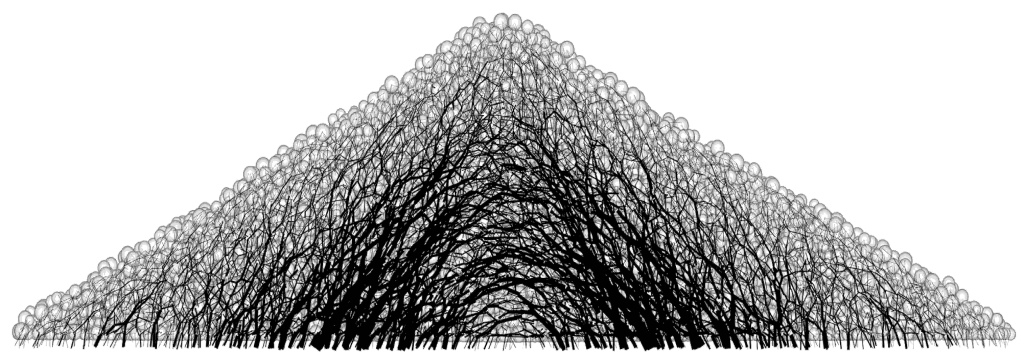
\includegraphics[width=0.9\textwidth]{force_chains.jpg}
    \caption{Силовая сеть в гранулированной насыпи}
    \label{fig:chainheap}
\end{figure}

Такое поведение объясняется полидисперсностью данного материала, за счет чего образуются силовые сети. Силовые сети состоят
из частиц внутри гранулированного материала под давлением, которые удерживаются вместе и заклиниваются сетью взаимных сжимающих сил. 
Между этими цепями находятся участки с низким напряжением, зерна которых "защищены" от воздействия вышеперечисленных зерен сводами и арками (рисунок \ref{fig:chainheap}). 
Набор взаимосвязанных силовых цепей известен как силовая сеть. Очевидно то, что такие полидисперсные материалы способны поглощать энергию и рассеивать ее
в дальнейшем, ведь зачастую такие материалы используются в качестве демпфирующих, но каким образом образующиеся силовые сети влияют на процессы поглощения 
и рассеивания энергии, а так же каким образом они формируются изучено еще недостаточно подробно. Изучение преобразования кинетической энергии поступательного
движения во внутреннюю энергию относительного движения в простейшей силовой цепи  представлено в данной работе.

\begin{figure}[h]
    \centering
    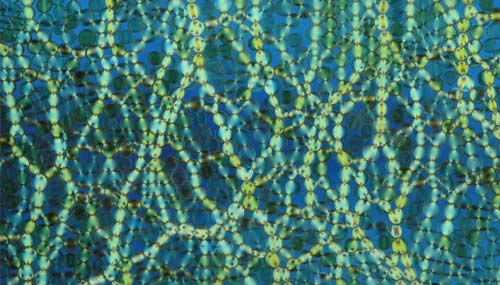
\includegraphics[width=0.9\textwidth]{chains1.jpg}
    \caption{Пример силовой сети полученной при нагружении фотоэластичных гранул}
    \label{fig:chainheap}
\end{figure}
\renewcommand{\thefigure}{\thechapter.\arabic{figure}}

\mainmatter % это включает нумерацию глав и секций в документе ниже
%КОНЦЕПТУАЛЬНАЯ ПОСТАНОВКА ЗАДАЧИ
%Постановка задачи
\newpage
\chapter{ПОСТАНОВКА ЗАДАЧИ}

\subsection*{Контактные силы в классической механике}
Согласно классической механике, когда к твердому телу применяется сила, центр масс тела
в соответствии со вторым законом Ньютона, начнет двигаться в направлении вектора
единицы силы с ускорением, равным отношению величины силы и массы тела.
Поскольку реальные тела не являются абсолютно жесткими, предположение, что все тело
будет двигаться с этим ускорением конечно неверно. В действительности приложенная
сила будет инициировать волны двигающиеся по телу, которые в конечном итоге приведут
к движению всего тела. Следовательно, важным вопросом является понимание перехода от
волновых процессов к движению объекта на макроуровне

Другой важный вопрос это разница/взаимосвязь между кинетической энергией волн,
распространяющихся внутри тела, и тепловой энергией тела, и переход от одного к другому.
Силы можно условно разделить на первичные и вторичные:

\begin{itemize}
\item \textbf{Первичные силы} - являются фундаментальной характеристикой материи и представляют собой силу
соответствующего потенциального энергетического поля, к которому они принадлежат.
В классической механике Ньютона мы как правило имеем дело с гравитационными и
электромагнитными силами. Действие сил всегда осуществляется посредством полей,
создаваемых телами и воспринимаемых рассматриваемым телом.
\item \textbf{Вторичные силы} - являются результатом взаимодействия вещества, поскольку для
возникновения требуют существования контакта между объектами, то есть являются
силами второго порядка.
\end{itemize}
В соответствии с третьим законом Ньютона действие одной силы способствует появлению
равной по модулю, но противоположной по направлению силы - пара сил.
При взаимодействии двух макроскопических объектов их атомы меняют свое положение
под действием соответствующих электромагнитных силовых полей, что в макромасштабе
наблюдается как деформации взаимодействующих объектов, что может быть постоянным
процессом, периодическим или их комбинацией.
Остающийся вопрос - как такое взаимодействие между двумя объектами может быть
обеспечено?

Контактные силы можно разделить на статические и динамические:
\begin{itemize}
\item \textbf{cтатические} - обусловленные первичными силами,
\item \textbf{динамические} - образованные в процессе включающем движение материи (динамический способ
генерации контактной силы / пары сил).
\end{itemize}

Взаимодействие двух тел, как было сказано выше, инициирует волны материи на микроуровне, 
которые в дальнейшем инициируют движение на макроуровне, то возникает вопрос, какая часть энергии, запасенной телом перейдет в 
поступательную кинетическую энергию тела? Аналогом такого взаимодействия может быть любое не абсолютно упругое взаимодействие 
двух тел, при котором часть энергии взаимодействия переходят во внутреннюю энергию тела, 
то есть в тепловую. Демпфирующие полидисперсные материалы так же являются аналогом такой системы и для демпфера важно 
эффективное преобразование кинетической энергии во внутреннюю энергию системы\cite{InfluenceOfNodes}.

Поведение гранулированных материалов может проходить через различные фазы, иметь
хаотичный характер, поэтому создание общей теории, описывающее поведение
гранулированных материалов, является затруднительным. При этом такие материалы могут поглощать
приложенную энергию колебаний, а ввиду возможности создания демпфирующих
элементов из прочных материалов с небольшим весом, они нашли применение в
высокотехнологичных отраслях: в работе \cite{work1} приводится пример применения
демпфирующих элементов, основанных на гранулированных материалах, в
аэрокосмической отрасли.

В данной работе также указано на тот факт, что при низких амплитудах вибрации, когда
частицы материала постоянно находятся в контакте, эффект демпфирования будет зависеть
от способности отдельных частиц к диссипации энергии. То есть можно анализировать
поведение материала под нагрузкой на основе анализа взаимодействия его отдельных
частиц.

Работа \cite{work1} также ссылается на аналитический метод, позволяющий найти эффективный
модуль упругости и эффективное отношение Пуассона случайной упаковки для одинаковых
упругих сфер, когда они находятся в постоянном контакте (аналог низкоамплитудной
вибрации), где постоянные сжимающие силы между любыми контактирующими
частицами могут быть вызваны гидростатическим сжатием вещества.

В научной литературе принято связывать процесс диссипации с переносом энергии
вещества из различных форм в тепловую.При этом возможны процессы, также потребляющие энергию, при действии которых
тепловая энергия незамкнутой системы будет меняться незначительно. Разумеется, в
конечном итоге энергия будет переходить в тепловую, но если ограничить
рассматриваемую область областью без диссипационных процессов, то можно
рассматривать диссипацию или поглощение энергии системой, не обусловленную
процессами трения и не связанные с выделением тепла.
Данная работа основана в большой степени на гипотезе Игоря Эмри, о том что
источниками диссипации энергии в определенных системах могут выступать контактные
силы, вследствии чего потребляемая системой энергия уходит не полностью в тепло, а
частично на создание силовой сети, засчет перераспределения волновой энергии взаимодействия тел. Данная гипотеза основана на экспериментах \cite{work2, work7} с
гранулированными материалами. 

С помощью экспериментальной установки \cite{work2} позволяющей исследовать поведение
материалов под давлением, как описано в работах \cite{work2, work7} было установлено что в
определенных условиях материал (полимерное вещество под давлением), поглощающий
энергию, изменяет свою температуру незначительно, т.е. не вся переданная веществу
энергия перешла в тепло в этом веществе. Этот эффект, как оказалось, практически не
исследован в литературе.

Среди исследований данной тематике можно привести работу \cite{work10} в которой с помощью
метода конечных элементов исследуются свойства гранулированных материалов
находящихся под нагрузкой. Результаты полученные численно для определенных
параметров системы не являются универсальными, следовательно не являются
достаточным результатом для анализа процессов поглощения энергии в демпфирующем
элементе.

Похожее исследование \cite{work11} изучает динамическое поведение механической системы с
одной степенью свободы содержащей демпфер частиц.
Результаты работы демонстрируют регулярное или хаотическое движение
гранулированного слоя при частоте возбуждения в качестве параметра управления.
Результаты демонстрируют поведение слоя вещества, но элементы трения в модели не
дают изучить требуемый эффект нетепловой диссипации.
Взаимосвязь диссипации энергии и образования пары сил или силовой сети в
гранулированных системах не изучена, а поскольку процессы диссипации могут иметь
практическое применение, было решено исследовать процесс, обуславливающий работу
демпфирующего элемента, то есть процесс диссипации энергии в гранулированных
материала.

Так же был произведен эксперимент, в котором по пластине из полидисперсного полимера заданной ширины стреляют пулей со скоростью 45 м/с, что приводит в разрушению пластины. Затем такой же пулей, с той же скоростью стреляют по пластине из того же полимера, но теперь ширина пластины уменьшена в два раза. 
В результате взаимодействия полимер не только не разрушается, но и останавливает пулю, что говорит о скрытых процессах внутри материала и влиянии процесса создания силовой сети на распространение деформаций и диссипацию энергии в материалах.

Таким образом для понимания процессов, происходящих в гранулированных материалах было решено проанализировать многоуровневый энергетический обмен в простейшей силовой сети и ее образования. Данный процесс рассматривается на двух различных уровнях: на внешнем - макроуровне(рисунок \ref{fig:micmac} (а) ), и на внутреннем - микроуровне(рисунок \ref{fig:micmac} (б) ). 

Простейшим примером взаимодействия на макроуровне является столкновение эластичного сферического тела массой $M$, которое движется с постоянной скоростью $v_0$, с жесткой стенкой. В процессе взаимодействия, согласно третьему закону Ньютона, между телом и жесткой стенкой сформируется пара сил: тело будет давить на стенку с силой $F$, а стенка будет давить на тело с силой $-F$. Последняя сила, в свою очередь, в течении времени $\Delta t$ остановит тело и ускорит его в обратном направлении со скоростью $-v_0$. Во время соударения внешняя кинетическая энергия будет превращена во внутреннюю потенциальную энергию эластичного тела. При этом многоуровневом взаимодействии и преобразовании энергии формируется контактная пара сил. Таким образом контактные силы являются результатом многоуровневого преобразования энергий.

Рассмотрим данный процесс на микроуровне. Представим тело в качестве системы нескольких тел с массами $m_1$, $m_2$, $m_3$, соединенных пружинами с жесткостями $k_2$, $k_3$, тогда внутренняя энергия системы будет заключена в кинетической энергии относительного движения частиц и энергии пружин. При этом взаимодействие тела с жесткой стенкой происходит посредством пружины жесткостью $k_1$. Преобразование энергий заключается в переходе внешней кинетической энергии движения масс, во внутреннюю энергию, аналогом которой в данной постановке задачи являются потенциальные энергии пружин, соединяющих массы, и кинетические энергии относительного движения масс. Таким образом, найдя энергию поступательного движения тела после соударения, мы можем узнать диссипацию энергии в системе, что не позволяет сделать анализ на макроуровне.

\begin{figure}[h]
    \begin{minipage}[h]{0.3\linewidth}
    \center{
        

\tikzset{every picture/.style={line width=0.75pt}} %set default line width to 0.75pt        

\begin{tikzpicture}[x=0.75pt,y=0.75pt,yscale=-1,xscale=1]
%uncomment if require: \path (0,244.3173065185547); %set diagram left start at 0, and has height of 244.3173065185547

%Straight Lines [id:da41391987557326315] 
\draw    (50.43,48.24) -- (50.43,234.24) ;


%Straight Lines [id:da8975629204988387] 
\draw    (50.43,70.24) -- (39.77,60.16) ;
\draw    (49.77,90.24) -- (39.1,80.16) ;
\draw    (50.43,110.24) -- (39.77,100.16) ;
\draw    (50.43,130.91) -- (39.77,120.83) ;


%Straight Lines [id:da3207421376516373] 
\draw    (51.1,150.91) -- (40.43,140.83) ;


%Straight Lines [id:da4433189705331644] 
\draw    (51.1,170.91) -- (40.43,160.83) ;


%Straight Lines [id:da1320019866862019] 
\draw    (50.43,191.58) -- (39.77,181.5) ;


%Straight Lines [id:da17396697635412584] 
\draw    (50.43,210.91) -- (39.77,200.83) ;


%Straight Lines [id:da7024410341299809] 
\draw    (49.77,228.91) -- (39.1,218.83) ;


%Shape: Circle [id:dp7508815890818632] 
\draw   (100,139) .. controls (100,125.19) and (111.19,114) .. (125,114) .. controls (138.81,114) and (150,125.19) .. (150,139) .. controls (150,152.81) and (138.81,164) .. (125,164) .. controls (111.19,164) and (100,152.81) .. (100,139) -- cycle ;
%Straight Lines [id:da41402643933373806] 
\draw    (114.31,102.16) -- (135.97,102.16) ;

\draw [shift={(112.31,102.16)}, rotate = 0] [fill={rgb, 255:red, 0; green, 0; blue, 0 }  ][line width=0.75]  [draw opacity=0] (8.93,-4.29) -- (0,0) -- (8.93,4.29) -- cycle    ;

% Text Node
\draw (126.67,86.67) node  [align=left] {$\displaystyle v_0$};
% Text Node
\draw (125,139) node  [align=left] {$\displaystyle M$};


\end{tikzpicture} \\ а)
    }
    \end{minipage}
    \hfill  
    \begin{minipage}[h]{0.3\linewidth}
    \center{
         

\tikzset{every picture/.style={line width=0.75pt}} %set default line width to 0.75pt        

\begin{tikzpicture}[x=0.75pt,y=0.75pt,yscale=-1,xscale=1]
%uncomment if require: \path (0,244.3173065185547); %set diagram left start at 0, and has height of 244.3173065185547

%Straight Lines [id:da41391987557326315] 
\draw    (50.43,48.24) -- (50.43,234.24) ;


%Straight Lines [id:da8975629204988387] 
\draw    (50.43,70.24) -- (39.77,60.16) ;


%Straight Lines [id:da4791030925335944] 
\draw    (49.77,90.24) -- (39.1,80.16) ;


%Straight Lines [id:da9564038647659947] 
\draw    (50.43,110.24) -- (39.77,100.16) ;


%Straight Lines [id:da6270302864150106] 
\draw    (50.43,130.91) -- (39.77,120.83) ;


%Straight Lines [id:da3207421376516373] 
\draw    (51.1,150.91) -- (40.43,140.83) ;


%Straight Lines [id:da4433189705331644] 
\draw    (51.1,170.91) -- (40.43,160.83) ;


%Straight Lines [id:da1320019866862019] 
\draw    (50.43,191.58) -- (39.77,181.5) ;


%Straight Lines [id:da17396697635412584] 
\draw    (50.43,210.91) -- (39.77,200.83) ;


%Straight Lines [id:da7024410341299809] 
\draw    (49.77,228.91) -- (39.1,218.83) ;


%Shape: Circle [id:dp7508815890818632] 
\draw   (70.76,153.62) .. controls (70.76,131.74) and (88.5,114) .. (110.38,114) .. controls (132.26,114) and (150,131.74) .. (150,153.62) .. controls (150,175.5) and (132.26,193.24) .. (110.38,193.24) .. controls (88.5,193.24) and (70.76,175.5) .. (70.76,153.62) -- cycle ;
%Straight Lines [id:da41402643933373806] 
\draw    (99.31,100.16) -- (120.97,100.16) ;

\draw [shift={(97.31,100.16)}, rotate = 0] [fill={rgb, 255:red, 0; green, 0; blue, 0 }  ][line width=0.75]  [draw opacity=0] (8.93,-4.29) -- (0,0) -- (8.93,4.29) -- cycle    ;
%Shape: Circle [id:dp6894624139524745] 
\draw   (84.85,153.62) .. controls (84.85,150.57) and (87.32,148.1) .. (90.37,148.1) .. controls (93.42,148.1) and (95.89,150.57) .. (95.89,153.62) .. controls (95.89,156.67) and (93.42,159.14) .. (90.37,159.14) .. controls (87.32,159.14) and (84.85,156.67) .. (84.85,153.62) -- cycle ;
%Shape: Circle [id:dp7196151672559912] 
\draw   (107.66,153.62) .. controls (107.66,150.57) and (110.13,148.1) .. (113.18,148.1) .. controls (116.23,148.1) and (118.7,150.57) .. (118.7,153.62) .. controls (118.7,156.67) and (116.23,159.14) .. (113.18,159.14) .. controls (110.13,159.14) and (107.66,156.67) .. (107.66,153.62) -- cycle ;
%Shape: Circle [id:dp6290232420684407] 
\draw   (132.06,153.62) .. controls (132.06,150.57) and (134.53,148.1) .. (137.58,148.1) .. controls (140.63,148.1) and (143.1,150.57) .. (143.1,153.62) .. controls (143.1,156.67) and (140.63,159.14) .. (137.58,159.14) .. controls (134.53,159.14) and (132.06,156.67) .. (132.06,153.62) -- cycle ;
%Straight Lines [id:da4539197689910155] 
\draw    (70.76,153.62) .. controls (72.43,151.95) and (74.09,151.95) .. (75.76,153.62) .. controls (77.43,155.29) and (79.09,155.29) .. (80.76,153.62) -- (84.85,153.62) -- (84.85,153.62) ;


%Straight Lines [id:da14488596850940327] 
\draw    (95.89,153.62) .. controls (97.56,151.95) and (99.22,151.95) .. (100.89,153.62) .. controls (102.56,155.29) and (104.22,155.29) .. (105.89,153.62) -- (107.66,153.62) -- (107.66,153.62) ;


%Straight Lines [id:da4969696424254402] 
\draw    (118.7,153.62) .. controls (120.37,151.95) and (122.03,151.95) .. (123.7,153.62) .. controls (125.37,155.29) and (127.03,155.29) .. (128.7,153.62) -- (132.06,153.62) -- (132.06,153.62) ;



% Text Node
\draw (111.67,84.67) node  [align=left] {$\displaystyle v_{0}$};
% Text Node
\draw (84.87,170.12) node [scale=0.5] [align=left] {$ $};
% Text Node
\draw (91.1,167.5) node [scale=0.9] [align=left] {$\displaystyle m_{1}$};
% Text Node
\draw (115,168.5) node [scale=0.9] [align=left] {$\displaystyle m_{2}$};
% Text Node
\draw (139.5,167.8) node [scale=0.9] [align=left] {$\displaystyle m_{3}$};


\end{tikzpicture}
 \\ б)
    }
    \end{minipage}
    \caption{Модель тела из полидисперсного материала на макроуровне (а) и на микроуровне (б)}
    \label{fig:micmac}
\end{figure}


%\begin{figure}[h]
%    \centering
%    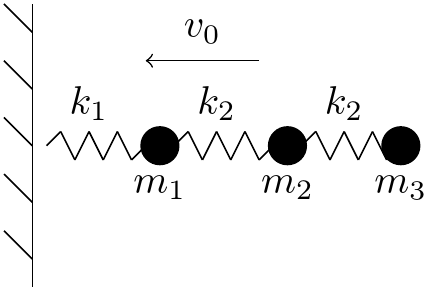
\includegraphics[width=0.4\textwidth]{sketch.png}
%    \caption{Эскиз системы трех тел. Все тела разделены пружинами длины $l$.}
%    \label{fig:sketch}
%\end{figure}


%МАТЕМАТИЧЕСКАЯ ПОСТАНОВКА ЗАДАЧИ

%Математическая модель
\chapter{МАТЕМАТИЧЕСКАЯ ПОСТАНОВКА ЗАДАЧИ}
\section{Математическая модель}

Система, показанная на рисунке \ref{fig:sketch} может быть описана следующей системой уравнений движения:
\begin{align}
	m_1 \ddot{x}_1 &= k_1 (l - x_1) - k_2 \left[ l - (x_2 - x_1) \right], \\
	m_2 \ddot{x}_2 &= k_2 \left[ l - (x_2 - x_1) \right] - k_3 \left[ l - (x_3 - x_2) \right], \\
	m_3 \ddot{x}_3 &= k_3 \left[ l - (x_3 - x_2) \right].
\end{align}
Сдвинув координаты, получим:
\begin{align}
	x_1 &= \tilde{x}_1 + l, \\
	x_2 &= \tilde{x}_2 + 2l, \\
	x_3 &= \tilde{x}_3 + 3l,
\end{align}
и, подставив полученные значения в уравнения движения, получим:
\begin{align}
	m_1 \ddot{\tilde{x}}_1 &= -k_1 \tilde{x}_1 + k_2 (\tilde{x}_2 - \tilde{x}_1), \\
	m_2 \ddot{\tilde{x}}_2 &= -k_2 (\tilde{x}_2 - \tilde{x}_1) + k_3 (\tilde{x}_3 - \tilde{x}_2), \\
	m_3 \ddot{\tilde{x}}_3 &= -k_3 (\tilde{x}_3 - \tilde{x}_2).
\end{align}
Разделив уравнения на соответствующие массы получим новые переменные: $\omega_i^2 = \frac{k_i}{m_i}$ and $\omega_{ij}^2 = \frac{k_i}{m_j}$. В итоге система уравнений имеет вид:
\begin{align}
	\ddot{\tilde{x}}_1 &= -\omega_1^2 \tilde{x}_1 + \omega_{21}^2 (\tilde{x}_2 - \tilde{x}_1), \\
	\ddot{\tilde{x}}_2 &= -\omega_2^2 (\tilde{x}_2 - \tilde{x}_1) + \omega_{32}^2 (\tilde{x}_3 - \tilde{x}_2), \\
	\ddot{\tilde{x}}_3 &= -\omega_3^2 (\tilde{x}_3 - \tilde{x}_2).
\end{align}
Для составления системы ОДУ введем вектор $q$:
\begin{equation}\label{eq:vector}
	\bm{q} = [q_1, q_2, q_3, q_4, q_5, q_6]^T = [\tilde{x}_1, \tilde{x}_2, \tilde{x}_3, \dot{\tilde{x}}_4, \dot{\tilde{x}}_5, \dot{\tilde{x}}_6]^T.
\end{equation}
Таким образом система ОДУ $\frac{d}{dt}q$ имеет вид:
\begin{equation}
	\frac{d}{dt}
	\begin{bmatrix} q_1 \\ q_2 \\ q_3 \\ q_4 \\ q_5 \\ q_6 \end{bmatrix}
	=
	\begin{bmatrix}
		0 & 0 & 0 & 1 & 0 & 0 \\
		0 & 0 & 0 & 0 & 1 & 0 \\
		0 & 0 & 0 & 0 & 0 & 1 \\
		-\omega_1^2 - \omega_{21}^2 & \omega_{21}^2 & 0 & 0 & 0 & 0 \\
		\omega_2^2 & -\omega_{2}^2 - \omega_{32}^2 & \omega_{32}^2 & 0 & 0 & 0 \\
		0 & \omega_{3}^2 & -\omega_{3}^2 & 0 & 0 & 0 \\
	\end{bmatrix}
	\begin{bmatrix} q_1 \\ q_2 \\ q_3 \\ q_4 \\ q_5 \\ q_6 \end{bmatrix}
	\label{eq:syst}
\end{equation}

Таким образом нахождение значений вектора $q$, путем решения ОДУ, позволяет найти значения скоростей и координат масс $m_1$, $m_2$, $m_3$ в любой момент времени и понять какие процессы протекают в системе во время взаимодействия.  
%Аналитическое решение
\section{Аналитическое решение}

Определитель матрицы $A$ равен $\omega_1^2 \omega_2^2 \omega_3^2$, что позволяет нам найти точное решение при помощи спектрального разложения.

\begin{equation}
	A=
	\begin{bmatrix}
		0 & 0 & 0 & 1 & 0 & 0 \\
		0 & 0 & 0 & 0 & 1 & 0 \\
		0 & 0 & 0 & 0 & 0 & 1 \\
		-\omega_1^2 - \omega_{21}^2 & \omega_{21}^2 & 0 & 0 & 0 & 0 \\
		\omega_2^2 & -\omega_{2}^2 - \omega_{32}^2 & \omega_{32}^2 & 0 & 0 & 0 \\
		0 & \omega_{3}^2 & -\omega_{3}^2 & 0 & 0 & 0 \\
	\end{bmatrix}	
\end{equation}

	Спектральное разложение имеет вид:
\begin{equation}
A = P^{-1} \Lambda P
\end{equation}
, где $A$ - изначальная матрица, $P$ - матрица собственных векторов, $\Lambda$- диагональная матрица, на диагонали которой расположены собственные числа матрицы $A$.
	Для данной задачи система ОДУ имеет вид: 
\begin{equation}
	\frac{d}{dt}q = A q
\end{equation}
	Применив спектральное разложения к матрице $A$, получим:
\begin{align}
	&\frac{d}{dt}q =  P^{-1} \Lambda P q,\\ 
	&\frac{d}{dt} P q =  \Lambda P q
\end{align}
	Произведем замену переменных $\tilde{q} = P q$. Теперь уравнение имеет вид:
\begin{equation}
	\frac{d}{dt}\tilde{q} = \Lambda \tilde{q}
\end{equation}
	Отсюда вектор $\tilde{q}$:
\begin{equation}\label{eq:q}
\tilde{q} = 
\begin{bmatrix}
 e^{\lambda_1 t} & & \\
    & \ddots & \\
    & & e^{\lambda_n t}
\end{bmatrix} \tilde{q}(0) ,
\end{equation}	
 где $t$ - время. В результате обратной замены получим $q = P^{-1} \tilde{q}$.

 Таким образом решение системы ОДУ сводится к нахождению собственных чисел матрицы $A$. Собственные числа можно найти аналитически, для этого запишем характеристический полином матрицы $A$:

\begin{multline}
	\lambda^6 + \lambda^4 ( \omega_{1}^2 + \omega_{2}^2 + \omega_{21}^2 + \omega_{3}^2 + \omega_{32}^2 ) + \lambda^2 (\omega_{1}^2 \omega_{2}^2 + \omega_{21}^2 \omega_{3}^2 + \omega_{21}^2\omega_{32}^2 + \omega_{3}^2 \omega_{2}^2 + \omega_{3}^2 \omega_{1}^2 +
	\omega_{32}^2 \omega_{1}^2) \\ + \omega_1^2 \omega_2^2 \omega_3^2 = 0\\
\end{multline} 
 Можно легко увидеть, что данное выражение легко сводится к кубическому уравнению вида:
 \begin{equation}
 	k^3 + k^2 W_1 + k W_2 + W_3 = 0 
 \end{equation}
, где 
 \begin{align}
 	&k = \lambda^2\\
 	&W_1 = \omega_{1}^2 + \omega_{2}^2 + \omega_{21}^2 + \omega_{3}^2 + \omega_{32}^2 \\
 	&W_2 = \omega_{1}^2 \omega_{2}^2 + \omega_{21}^2 \omega_{3}^2 + \omega_{21}^2\omega_{32}^2 + \omega_{3}^2 \omega_{2}^2 + \omega_{3}^2 \omega_{1}^2 +
	\omega_{32}^2 \omega_{1}^2\\
	&W_3 =  \omega_1^2 \omega_2^2 \omega_3^2
 \end{align}

Решим данное уравнение при помощи тригонометрической формулы Виета для кубического уравнения:

\begin{align}
	&Q = \frac{W_1^2 - 3 W_2}{9}\\
	&R = \frac{2 W_1^3 - 9 W_1 W_2 + 27 W_3}{54}\\
	&S = Q^3 - R^2
\end{align}

Если $S>0$, то имеем три действительных корня, вычисляемых при помощи тригонометрических функций. При $S<0$, тригонометрические функции заменяются на гиперболические и пара корней является комплексными. При $S=0$ уравнение вырождено и имеет два корня.
Программная реализация решателя на языке Python, использующего тригонометрическую формулу Виета, представлена в листинге \ref{lst:viett}.

\newpage
\begin{lstlisting}[numbers=none, label=lst:viett,language=Python, caption=Программная реализация решателя кубического уравнения при помощи теоремы Виета]
def cbslv(a, b, c):
	Q = (a**2 - 3*b)/9
	R = (2*a**3 - 9*a*b+27*c)/54
	S = Q**3 - R**2
	if S > 0:
		phi = cmt.acos(R/cmt.sqrt(Q**3))/3
		x1 = -2*cmt.sqrt(Q)* cmt.cos(phi) - a/3
		x2 = -2*cmt.sqrt(Q+2*np.pi/3)* cmt.cos(phi) - a/3
		x3 = -2*cmt.sqrt(Q-2*np.pi/3)* cmt.cos(phi) - a/3
	elif S < 0:
		if Q > 0:
			phi = cmt.acosh(abs(R)/cmt.sqrt(Q**3))/3
			x1 = -2*np.sign(R)*cmt.sqrt(Q)*cmt.cosh(phi) - a/3 # real root
			x2 = np.sign(R)*cmt.sqrt(Q)*cmt.cosh(phi) - a/3 + 1j*cmt.sqrt(3)*cmt.sqrt(Q)*cmt.sinh(phi)
			x3 = np.sign(R)*cmt.sqrt(Q)*cmt.cosh(phi) - a/3 - 1j*cmt.sqrt(3)*cmt.sqrt(Q)*cmt.sinh(phi)
		elif Q < 0:
			phi = cmt.asinh(abs(R)/cmt.sqrt(abs(Q)**3))/3
			x1 = -2*np.sign(R)*cmt.sqrt(abs(Q))*cmt.sinh(phi) - a/3 # real root
			x2 = np.sign(R)*cmt.sqrt(abs(Q))*cmt.sinh(phi) - a/3 + 1j*cmt.sqrt(3)*cmt.sqrt(abs(Q))*cmt.cosh(phi)
			x3 = np.sign(R)*cmt.sqrt(abs(Q))*cmt.sinh(phi) - a/3 - 1j*cmt.sqrt(3)*cmt.sqrt(abs(Q))*cmt.cosh(phi)
		elif Q == 0:
			x1 = -np.cbrt(c-(a**3)/27) - a/3
			x2 = -(a+x1)/2 +1j/2*cmt.sqrt(abs((a - 3*x1)*(a+x1)-4*b))
			x2 = -(a+x1)/2 -1j/2*cmt.sqrt(abs((a - 3*x1)*(a+x1)-4*b))
	elif S==0:
		x1 = -2*np.cbrt(R)-a/3
		x2 = np.cbrt(R)-a/3
		x3 = None
	return x1, x2, x3
\end{lstlisting}

Изначальной идеей нахождения аналитического решения было избавление от переменных и от большого количества арифметических операций. Это могло позволить найти прямые зависимости состояний системы от каких либо из ее параметров. Но в ходе подстановки не удалось сократить какие либо переменные, а вкупе с использованием ресурсозатратных гиперболических функций и вычислением сложных степеней больших чисел аналитическое решение приводит к ошибкам вычислений и отклонениям. А так же к большему времени расчетов, относительно численных методов.

%ВЫЧИСЛИТЕЛЬНЫЙ МЕТОД
%Численное решение
\chapter{ВЫЧИСЛИТЕЛЬНЫЙ МЕТОД}
\section{Метод Рунге-Кутта 4-го порядка}

 В связи с тем, что точное решение имеет большую вычислительную сложность, то воспользуемся методом Рунге-Кутта 4-го порядка для решения системы ОДУ\cite{BahvalJidkovKobel1987}. Согласно методу приближенное значение в последующих точках вычисляется по итерационной формуле:

\begin{equation}
	y_{i+1} = y_i + \frac{h}{6} (k_1 + 2 k_2 + 2 k_3 + k_4)
\end{equation} 

Коэффициенты в общем виде находятся по формулам:

\begin{align}
	&k_1= f(x_i, y_i)\\
	&k_2=f(x_i + \frac{h}{2}, y_i + \frac{h}{2}k_1)\\
	&k_3=f(x_i + \frac{h}{2}, y_i + \frac{h}{2}k_2)\\
	&k_4 =  f(x_i + h, y_i + h k_3)\\
\end{align}, где $h$ - величина шага сетки по $x$.

Относительно задачи, рассматриваемой в данной работе аналогом $x$ является время $t$. А аналогом $y$ - вектор $q$, описывающий состояние системы  (\ref{eq:vector}). Тогда уравнение $\frac{d}{dt}q = f(t, q)$ принимает вид (\ref{eq:syst}). Начальные условия задачи Коши нам известны из постановки задачи. 
Легко можно заметить, что по сравнению с аналитическим решением, в методе Рунге-Кутта требуется произвести меньшее количество арифметических операций, что критично для данной задачи, потому что требуется проводить анализ большого количества возможных состояний системы, а это значит каждый раз симулировать процесс. А вкупе с тем что данный численный метод имеет порядок точности $O(h^4)$, то было решено использовать данный метод для получения приближенных значений состояний системы для каждого момента времени. На рисунке \ref{fig:anchi} продемонстрированы графики зависимости состояния системы от времени для параметров $k_1 = k_2 = k_3 = 1.5$ и $m_1 = m_2 = m_3 = 1$ со значением шага $h=0.01$с, что дает в итоге точность $O(h^4) = 10^{-8}$. На основе графиков и порядка точности можно сделать вывод, что данной точности интегрирования достаточно для решения поставленной задачи.

\begin{figure}[h]
    \begin{minipage}[h]{0.5\linewidth}
    \center{
        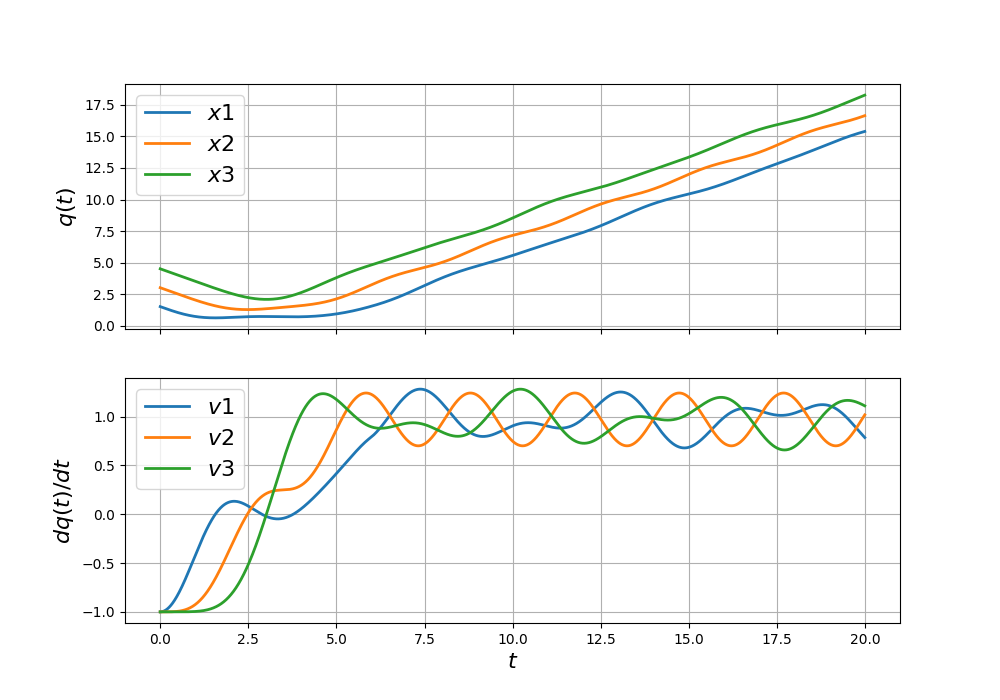
\includegraphics[width=1\textwidth]{analittraject.png} \\ a)
    }
    \end{minipage}
    \hfill  
    \begin{minipage}[h]{0.5\linewidth}
    \center{
         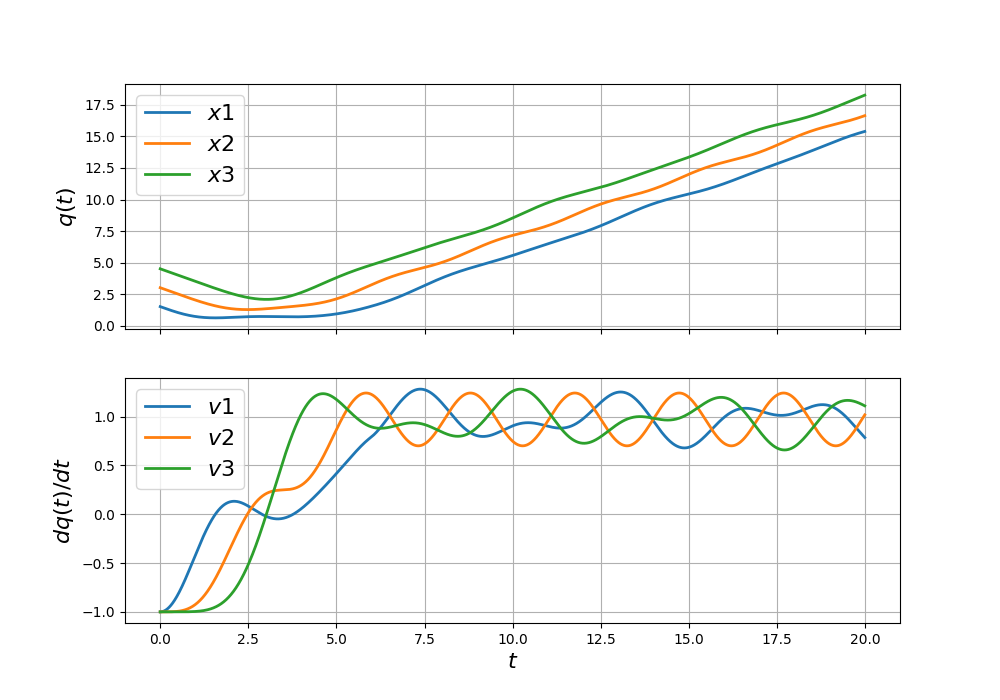
\includegraphics[width=1\textwidth]{rk4taject.png} \\ б)
    }
    \end{minipage}
    \caption{Траектории скоростей и координат системы трех тел, полученные аналитически (a) и численно (б) .}
    \label{fig:anchi}
\end{figure}
%Конечный автомат
\section{Конечно-автоматная модель}

 Так как система тел при движении во времени может принимать несколько состояний, то мы можем рассмотреть данную систему в качестве  конечного автомата с тремя возможными состояниями, описывающий динамическое состояние системы. Всего возможно три состояния системы:
\begin{enumerate}
	\item тело взаимодействует со стенкой;
	\item тело не взаимодействует со стенкой (свободное движение);
	\item нефизический случай.
\end{enumerate}

При наличии взаимодействия со стенкой в уравнении появляется пара сил: сила упругости первой пружины $F$ и, согласно третьему закону Ньютона действует обратная сила со стороны стенки.Ппри отсутствии взаимодействия, очевидно, данная пара сил не существует, поэтому в состоянии оторванном от стенки считается, что первая пружина отсутствует. Взаимодействие со стенкой происходит, когда значение координаты массы $m_1$ меньше или равняется длине пружины  $l$ в ненапряженном состоянии.

 Нефизическим случаем является такое состояние системы, при котором значение координаты массы $m_{i+1}$ становятся меньше значения координаты массы $m_i$,изначально находящейся ближе к стенке. Также нефизическим случаем является, когда значение координаты какой-либо массы становиться меньше 0 (масса "прошла" сквозь стенку). Граф, описывающий конечный автомат, представлен на рисунке 
 \ref{fig:avtomat}. Программная реализация автомата представлена на блок-схеме \ref{fig:konavtbs}.


\newpage
\begin{figure}
    \centering
    \scalebox{0.5}{\begin{tikzpicture}[start chain=going below,node distance=6mm, column sep=2cm]
    \node [cloud] (start) {Начало};
    \node [block, join] (init1) {Задание начальных значений};
    \node [block, join] (init2) {State := STARTED};

    \node [cyclebegin, join] (cycbeg) {time = 0; time <= tfin};
    \node [subroutine, join] (chck) {Проверка\\ состояния};
    \node [block, join] (stat) {State = Current State};
    \node [block, join] (step) {Вычисление значений\\ скоростей и координат\\ на следующем шаге};
    \node [io, join] (write ) {Вывод полученных\\ значений в файл};
    \node [cycleend, join] (cycend) {time+=time step};
    
    \node [cloud, join] (finish) {Конец};
\end{tikzpicture}}
    \caption{Блок-схема, описывающая программную реализацию конечного автомата}
    \label{fig:konavtbs}
\end{figure}

\begin{figure}
    \centering
    \scalebox{0.6}{\begin{tikzpicture}[shorten >=1pt,node distance=5cm,on grid, auto, scale=0.2] 
        \node[state,initial] (q_0) {
            \begin{tabular}{c}
                Свободное \\ движение тела
            \end{tabular}
        };
        \node[state] (q_1) [right=of q_0] {
            \begin{tabular}{c}
                Тело \\ взаимодействует \\со стенкой
            \end{tabular}
        };
        \node[state] (q_2) [below=of q_0] {
            \begin{tabular}{c}
                Нефизический\\ случай
            \end{tabular}
        };
        \path[->, bend right = 30] (q_0) edge node [below] {$x_1 \leq l$} (q_1);
        \path[->, bend right = 30] (q_1) edge node [above] {$x_1 > l$} (q_0);
        \path[->, bend right = 30] (q_0) edge node [left] {
            \begin{tabular}{c}
                $x_2\leq x_1$, \\
                $x_3\leq x_2$, \\
                $x_1\leq 0$  \\
            \end{tabular}
        } (q_2);
        \path[->, bend left = 30] (q_1) edge node [below right] {
           \begin{tabular}{c}
                $x_2\leq x_1$ \\
                $x_3\leq x_2$ \\
                $x_1\leq 0$  \\
            \end{tabular}
        } (q_2);
    \end{tikzpicture}}
    \caption{Конечный автомат, описывающий динамическое состояние системы трех масс, взаимодействующих со стенкой}
    \label{fig:avtomat}
\end{figure}


%ПРОГРАММНАЯ РЕАЛИЗАЦИЯ
\chapter{ПРОГРАММНАЯ РЕАЛИЗАЦИЯ}
\section{Используемые программные средства}

В данной работе было использованы следующие языки программирования:
\begin{itemize}
    \item Python
    \item Golang
\end{itemize}

Изначально все математические модели были реализованы на языке Python с использованием библиотеки numpy, это было сделано для проверки их работоспособности. Несомненным приемуществом работы Python является его простота в использовании, а так же большое количество готовых библиотек, сильно 
упрощающих разработку. Но так же Python является языком динамической типизации, что значительно влияет на скорость его работы, поэтому для задач,
требующих больших вычислительных мощностей, которой как раз и является данная задача, использование Python является нецелесообразным. Поэтому дальнейшая
разработка производилась на языке Golang.

\subsection*{Язык Golang}

Среди современных языков программирования следует выделить язык программирования Go, реализация которого была выполнена командой разработчиков фирмы Google \cite{GoTour}. Язык Go разрабатывался как язык программирования для создания высокоэффективных программ, работающих на современных распределённых системах и многоядерных процессорах. Он может рассматриваться как попытка создать замену языкам Си и C++. 

Основные возможности Golang:
\begin{itemize}
    \item Go — язык со строгой статической типизацией. Доступен автоматический вывод типов, для пользовательских типов — "утиная типизация".
    \item Полноценная поддержка указателей, но без возможности применять к ним арифметические операции, в отличие от C/C++/D.
    \item Использование динамических массивов, хеш-таблиц, срезов (слайсов), вариант цикла для обхода коллекции.
    \item Средства функционального программирования: неименованные функции, замыкания, передача функций в параметрах и возврат функциональных значений.
    \item Автоматическое управление памятью со сборщиком мусора.
    \item Средства объектно-ориентированного программирования, но без поддержки наследования реализации (наследуются только интерфейсы). По большому счёту, Go является процедурным языком с поддержкой интерфейсов.
    \item Средства параллельного программирования: встроенные в язык потоки (go routines), взаимодействие потоков через каналы и другие средства организации многопоточных программ.
    \item Достаточно лаконичный и простой синтаксис, основанный на Си.
\end{itemize}

Go содержит конструкцию, которая позволяет запустить исполнение вызова некоторой функции в отдельном потоке. Такая функция называется в Go горутиной (англ. goroutine), ниже приведен пример оператора вызова горутины: 

\begin{lstlisting}[numbers=none, language=Golang, caption=Пример вызова горутины]
    go f(args) 
\end{lstlisting} 

Каналы используются в качестве средства взаимодействия между горутинами. Помимо каналов в пакете \textit{sync} содержатся такие примитивы синхронизации, как мьютексы или условные переменные, однако их рекомендуется применять только для низкоуровневых библиотек.

Каналы в Go типизированы и являются объектами первого класса. Их можно посылать в функции, возвращать из функций, присваивать переменным и полям структур, а также пересылать по каналам. Они могут работать только в одну сторону или в обе. Причем, если обычный двунаправленный канал передать в функцию, где он используется, например, только на прием, его можно промаркировать соответствующим образом в списке параметров функции и компилятор проверит правильность его использования. Обычные каналы блокируют горутину, которая пытается получить из или послать что-то в канал, пока с другой стороны не будет произведено соответсвующее обратное действие. Но канал может иметь буфер, который может накапливать и отдавать накопленное определенное количество значений без блокировки. Канал может быть закрыт встроенной функцией \textit{close}, после этого посылка в него значений приведет к "панике", так в данном языке называется экстренное завершение программы в случае ошибки. Если закрытый канал имеет непустой буфер, эти значения все еще могут быть получены. Но когда буфер уже пуст или его нет, закрытый канал при попытке чтения будет выдавать нулевые значения того типа, для пересылки которых он создан. То есть, закрытый строковый канал будет выдавать пустые строки, целочисленный — нули, канал указателей — nil. Более подробно горутины и в целом язык Golang описывается в книге \cite{ProgrammingInGo}

Также неоспоримым приемуществом Golang является его скорость работы и компиляции, сопоставимая с такими языками, как Java, C, C++. На рисунке \ref{fig:govs} сопоставлены популярные языки и Go, на примере часто встречающихся задач.

\begin{figure}[h]
    \centering
    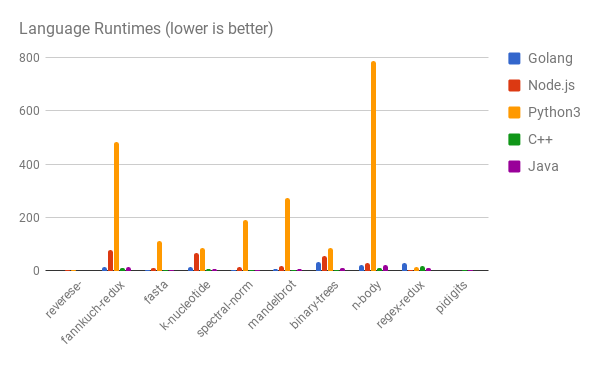
\includegraphics[width=0.9\textwidth]{golang-language-runtimes-1.png}
    \caption{Сопоставление Golang, Python, C++, Java, Node.js.}
    \label{fig:govs}
\end{figure}

Учитывая наличие сборщика мусора, времени компиляции сопоставимым с C++, а так же простотой синтаксиса и читабельностью кода, было решено остановиться на данном языке как на основном языке разработки. Так же в Golang есть возможноть исполнения кода, написанного на языке C, что позволяет уменьшить время работы программ, а так же использовать математические библиотке blas и lapack, которые реализованы в пакете \textbf{gonum}\cite{GoNum}. 
\section{Параллелизация вычислений}

Задача параллелизации представляет собой программное ускорение расчета полей накопленных энергий после соударения системы трех тел со стенкой в зависимости
от конфигурации системы. Расчет энергий происходит путем моделирования взаимодействия тел, что представляет собой решение системы ОДУ для каждого момента
времени при помощи метода Рунге-Кутта 4 порядка \cite{BahvalJidkovKobel1987}. Для понимания какой из параметров вносит больший вклад в накопление энергии 
требуется провести большое количество симуляций, которые линейно влияют на время расчетов. Было решено использовать возможности языка Golang, для программного
ускорения времени расчетов и более полного использования ресурсов компьютера, а в дальнейшем и вычислительного кластера.

Для ускорения вычисления были реализованы функции считающие двумерные поля(листинг \ref{lst:2d}) и трехмерные облака точек(листинг \ref{lst:3d}).
Обе функции используют все ядра центрального процессора.



Параллелизация работы в случае функции представленной в листинге \ref{lst:3d} достигается за счет того, что на каждую горутину выделяется одна плоскость в трехмерном пространстве, 
которую необходимо расчитать, после окончания расчета по каналу отправляется строковая переменная содержащая в себе данные расчетов, полученные данной горутиной.

Параллелизация работы в случае функции представленной в листинге \ref{lst:2d} достигается, за счет разделения плоскости расчетов между всеми доступными ядрами процессора,
что позволяет параллельно производить несколько симуляций. Во время расчетов, аналогично трехмерному случаю формируется строковая переменная, которая отправляется по каналу.


\begin{lstlisting}[numbers=none, label=lst:bar,language=Golang, caption=Функция барьер][t]
    func barrier(nrouts int, ch chan string, fil *os.File) {
        for r := 0; r < nrouts; r++ {
            x := <-ch
            log.Println("goroutine ", r, "writed", len(x))
            fil.WriteString(x)
        }
    }
\end{lstlisting}

Полученные через канал строки обрабатываются в функции представленной в листинге \ref{lst:bar}. Данная функция принимает по каналу определенное количество переменных типа строка,
которое равно число запущенных горутин, тем самым реализует работу барьера и блокирует выполнение родительской горутины до завершения работы всех дочерних горутин.
После строковая переменная записывается в файл для дальнейшей визуализации.
\section{Взаимодействие с кластером}

В современных задачах зачастую возникают задачи предъявляющие высокие требования к аппаратным мощностям, которые не всегда
могут быть доступны. Зачастую в таком случае прибегают к работе с удаленной машиной, обладающей достаточной вычислительной мощностью,
чтобы удовлетворить требования. Очевидным решением для облегчения взаимодействия конечного пользователя и ПО является клиент-серверное
приложение. Данный подход позволит свести взаимодействие конечного пользователя с исходным кодом программ к минимуму.

В данной работе для работы с серверной частью был использован язык Golang, а в частности пакет \textbf{gin-gonic} \cite{GinGonic}, который является веб-фреймворком,
предоставляющий более быструю работу чем стандартный сетевой пакет. Основной частью пакета является роутер, определяющий
какой запрос пришел со стороны клиента. Разработчик же описывает каким образом должен реагировать сервер на тот или иной запрос, 
путем назначения функций обработчиков на различные варианты запросов. Golang не требует установки какого либо дополнительного программного обеспечения 
для реализации сервера(например Apache), все эти функции уже есть в стандартном сетевом пакете.

Клиентский интерфейс содержит в себе следующие страницы:
\begin{enumerate}
    \item Главная страница
    \item Симуляция системы трех тел
    \item Вычисление двумерного поля энергий
    \item Вычисление трехмерного облака точек
    \item Результаты симуляций
    \item Страница ошибки
\end{enumerate}

Данные страницы реализованы на языке html и формируют GET или POST запросы на сервер. Страницы 2,3,4 -  содержат в себе поля для ввода параметров симуляции 
и интегрирования, которые формируют POST запрос и на сервере, который представляет собой кластер, обрабатываются и запускают симуляцию.  В листинге \ref{lst:post}
реализован парсинг формы запроса, получение даннных, требующихся для запуска симуляции и непосредственно запуск симуляции. 


\begin{lstlisting}[numbers=none, language=Golang,caption=Реализация обработчика POST запроса, label=lst:post]
    r.POST("/sim", func(c *gin.Context) {
		var m [3]float64
		m[0], _ = strconv.ParseFloat(c.PostForm("m1"), 64)
		m[1], _ = strconv.ParseFloat(c.PostForm("m2"), 64)
		m[2], _ = strconv.ParseFloat(c.PostForm("m3"), 64)

		var k [3]float64
		k[0], _ = strconv.ParseFloat(c.PostForm("k1"), 64)
		k[1], _ = strconv.ParseFloat(c.PostForm("k2"), 64)
		k[2], _ = strconv.ParseFloat(c.PostForm("k3"), 64)

		v, _ := strconv.ParseFloat(c.PostForm("vel"), 64)
		l, _ := strconv.ParseFloat(c.PostForm("len"), 64)

		step, _ := strconv.ParseFloat(c.PostForm("stpt"), 64)
		fint, _ := strconv.ParseFloat(c.PostForm("fint"), 64)

		c.Redirect(301, "/dat")
		avg := c.Request.FormValue("avg")

		body := slv.NewThreeBodyModel(m, k)
		//y, mon, d := time.Now().Date()
		filename := fmt.Sprintf("sym%v.dat", time.Now().Format("15:04:05_02Jan06"))
		file, err := os.Create(fmt.Sprint("./dat/", filename))
		if err != nil {
			log.Println("Cannot create file!  :", err)
			c.File("./www/error.html")
			return
		}

		machine := slv.StateMachFromModel(body, v, l, step, 0, fint)
		if avg == "on" {
			go func(machine grn.StateMachine, body grn.ThreeBodyModel, file *os.File, filename string) {
				filsys[filename] = false
				slv.SimulateAv(machine, body, file)
				filsys[filename] = true
			}(machine, body, file, filename)

		} else {
			go func(machine grn.StateMachine, file *os.File, filename string) {
				filsys[filename] = false
				time.Sleep(30 * time.Second)
				slv.Simulate(machine, file)
				filsys[filename] = true
			}(machine, file, filename)
		}
	})
\end{lstlisting}

Симуляция запускается отдельной горутиной, что позволяет работать серверу и расчетному ПО параллельно и не останавливать работу сервера. Также для реализации 
отслеживания процесса расчетов был реализован ассоциативный массив \textit{filsys}, который содержит текущее состояние для каждого файла симуляции, где имя файла является ключом, 
а значение отображает состояние файла, если значение \textit{false}, то вычисление данного файла еще не закончено, иначе файл может быть загружен с кластера для дальнейшей 
визуализации.

Страница 5, формируется динамически сервером, в зависимости от состояния файла \textit{filsys}. Для автоматической генерации html страницы используется 
пакет \textit{template}, который позволяет формировать страницу в зависимости от контекста.

\begin{lstlisting}[numbers=none, language=html,caption=Html шаблон, label=lst:templ]
    <!DOCTYPE html>
    <html>
    <head>
        <meta charset="UTF-8" />
    </head>
    <body>
        <div>
            <p><h2>Simulation results</h1></p>
            <hr>
            {{ range $key, $value := . }}
                <li>
                    {{ $key }}
                    {{if $value }}
                        <form method="POST" action="/dat">
                            <input name="file" type="hidden" value="{{ $key }}"><input type="submit"  value="Download">
                        </form>
                    {{else}}
                        <strong>File in progress...</strong>
                    {{end}}
                </li>
            {{ end }}
        </div>
        <a href="/">Back to menu</a>
    </body>
    </html>
\end{lstlisting}

Шаблон в листинге \ref{lst:templ}, формирует страницу в зависимости от значений \textit{filesys}, \textit{range  \$key, \$value := . } - цикл, 
который перебирает все ключи и значения, переданные программой, формирующей страницу(листинг \ref{lst:frm}). В зависимости от значений \textit{\$value}, формируется либо сообщение
о том что файл еще рассчитывается, либо форма POST запроса со скрытым полем, содержащим имя файла. При нажатии на кнопку выбранный файл расчетов скачивается
с кластера на клиентскую машину.

\begin{lstlisting}[numbers=none, language=html,caption=Формирование html, label=lst:frm]
r.GET("/dat", func(c *gin.Context) {
		t, err := template.ParseFiles("./www/dat.html")
		if err != nil {
			panic(err)
		}

		err = t.Execute(c.Writer, filsys)
		if err != nil {
			panic(err)
		}
    })
\end{lstlisting}

\newpage
\begin{figure}[h]
    \centering
    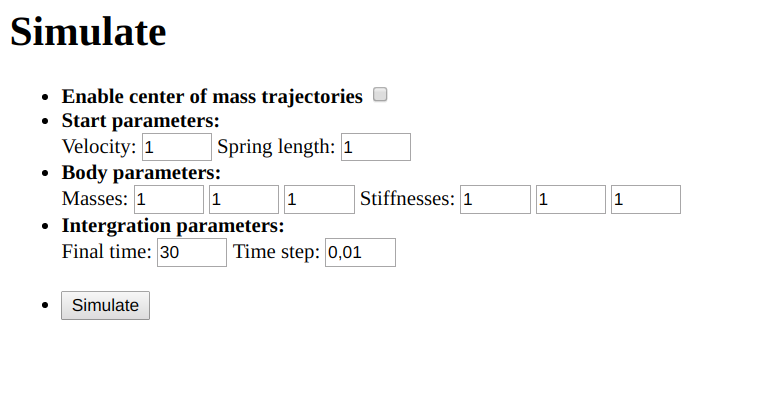
\includegraphics[width=0.7\textwidth]{net/scren1.png}
    \caption{Зависимость $\Delta \tilde{E}$ от различных значений масс. Каждый график соответствует одной переменной массе.}
\end{figure}

\newpage
\begin{figure}[h]
    \centering
    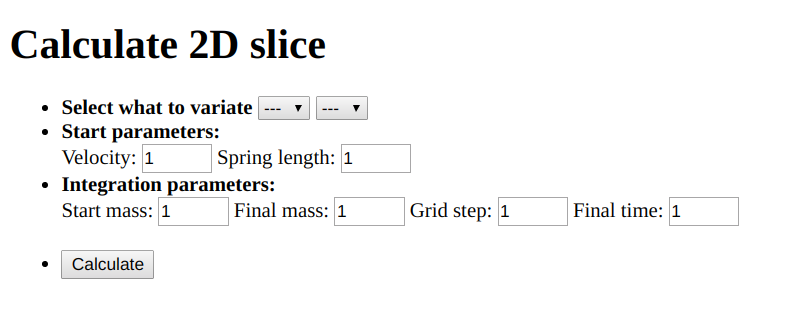
\includegraphics[width=0.7\textwidth]{net/scren2.png}
    \caption{Зависимость $\Delta \tilde{E}$ от различных значений масс. Каждый график соответствует одной переменной массе.}
\end{figure}

\newpage

\begin{figure}[h]
    \centering
    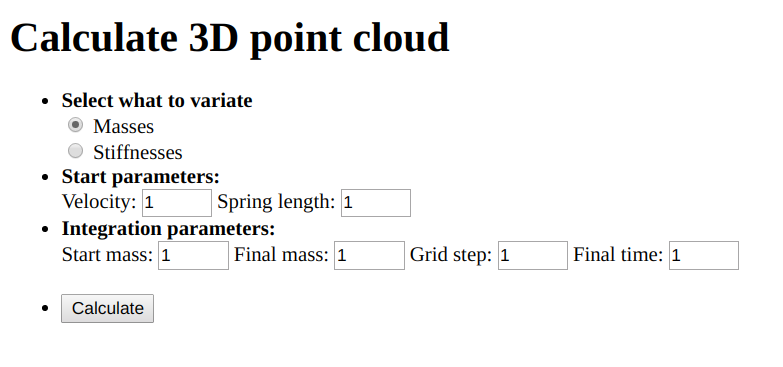
\includegraphics[width=0.7\textwidth]{net/scren3.png}	
    \caption{Зависимость $\Delta \tilde{E}$ от различных значений масс. Каждый график соответствует одной переменной массе.}
\end{figure}

%ВЫЧИСЛИТЕЛЬНЫЙ ЭКСПЕРИМЕНТ

%TODO:Анализ результатов
\chapter{ВЫЧИСЛИТЕЛЬНЫЙ ЭКСПЕРИМЕНТ}
%\section{Вычислительный эксперимент}

Основным вопросом, поставленным в данной работе является нахождение таких состояний системы трех тел, что внутренняя энергия, запасенная в пружинах будет максимальна или минимальна. А так же нахождение таких состояний, при которых внутренняя энергия тела после соударения равна 0 или же наоборот вся вся кинетическая энергия перейдет во внутреннюю.

Для нахождения потерь энергии во время взаимодействия запишем Закон сохранения энергии:
\begin{equation}\label{eq:energy}
    \frac{M v_0^2}{2} = \frac{m_1 v_1^2}{2} + \frac{m_2 v_2^2}{2} + \frac{m_3 v_3^2}{2} + \frac{k_2 \Delta l^2}{2} + \frac{k_3 \Delta l^2}{2}
\end{equation}, где $M = m_1 + m_2 + m_3$. Энергия, накопленная первой пружиной отсутствует, так как вся энергия пружины переходит в ускорение тел и растяжение и сжатие остальных пружин.

Так как нас интересует потери энергии для тела на макроуровне, то рассмотрим систему трех тел после соударения как единое тело с постоянной скоростью, тогда разница между кинетическими энергиями до и после соударения и будет показывать накопленную внутреннюю энергию тела. Для этого запишем уравнение для скорости центра масс:

\begin{equation}
    v_c = \frac{m_1 v_1 + m_2 v_2 + m_3 v_3}{M}
\end{equation}
, тогда Закон сохранения энергии примет вид:

\begin{equation}
    \frac{M v_0^2}{2} = \frac{M v_c^2}{2} + \Delta E
\end{equation}
, где $\Delta E$ - энергия накопленная в пружинах и кинетическая энергия движения масс относительно центра масс.


\begin{figure}[b!]
    \centering
    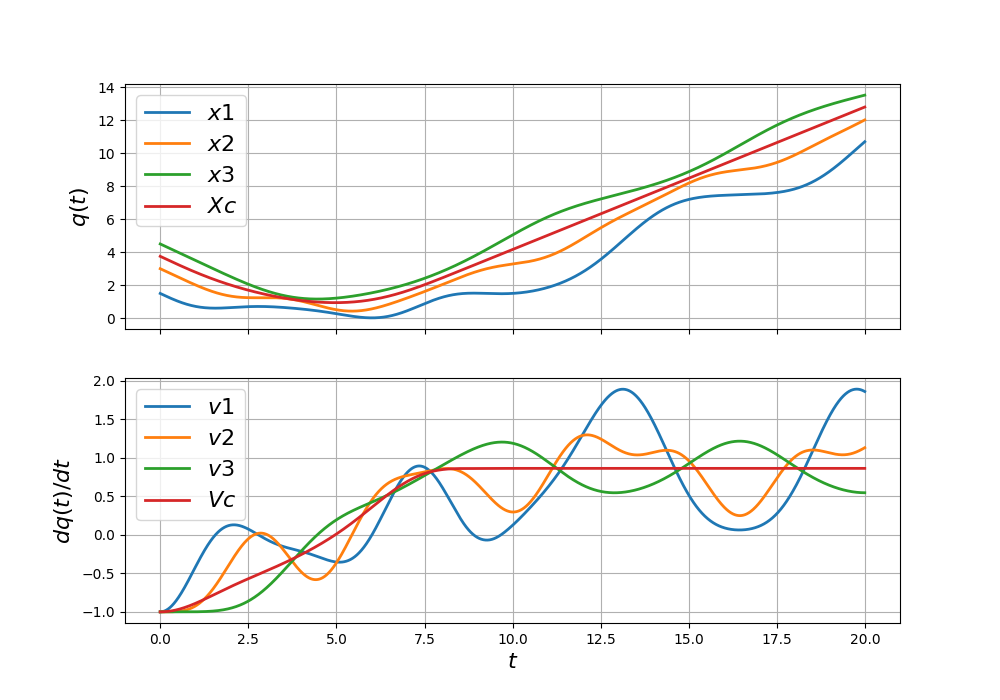
\includegraphics[width=0.7\textwidth]{snaps_midd.png}
    \caption{График координат и скоростей тел на микроуровне и на макроуровне(красным).}
    \label{fig:snapmidd}
\end{figure}

На рисунке \ref{fig:snapmidd} на графике продемонстрирован результат симуляции с нахождением скорости центра масс, а так же его координат, из чего можно сделать вывод что после взаимодействия часть кинетической энергия тела перешла во внутреннюю энергию тела, соответственно скорость тела после соударения уменьшилась. Массы для данной симуляции заданы следующим образом: $m_1 = m_2 = 1; m_3 = 4$. Начальная скорость $v_0$=1м/с. При этом можно увидеть, что итоговая скорость тела после взаимодействия меньше первоначальной, засчет преобразования энергий. Энергия, перешедшая во внутреннюю и есть искомая $\Delta E$.

Проведем вычислительный эксперимент с различными входными параметрами системы (длина пружин $l=1$). Для определения параметра, в большей степени влияющего на состояние системы измерим $\Delta E$ для каждого параметра в некоторых пределах. Но очевидно что, например, большая масса способна сильней повлиять на численное значение $\Delta E$. Тогда введем $\Delta \tilde{E} = \frac{\Delta E}{E_0}$, где $E_0$ - изначальная энергия системы. $\Delta \tilde{E}$ - коэффициент эффективности диссипации энергии. Для случая представленного на рисунке \ref{fig:snapmidd} $\Delta \tilde{E} = 27.26\%$. На графиках на рисунке \ref{fig:deltas} продемонстрированы зависимость коэффициента эффективности диссипации от различных масс.


\begin{figure}[b!]
    \centering
    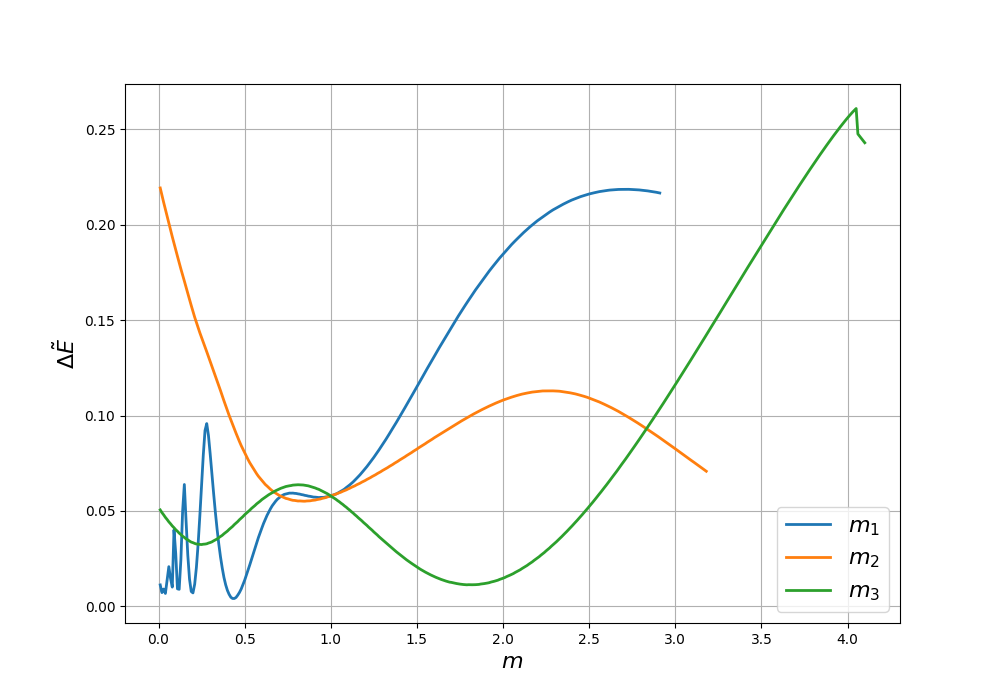
\includegraphics[width=0.7\textwidth]{deltas.png}
    \caption{Зависимость $\Delta \tilde{E}$ от различных значений масс. Каждый график соответствует одной переменной массе.}
    \label{fig:deltas}
\end{figure}

Аналогичный эксперимент проведем для переменных жесткостей пружин:

\begin{figure}[b!]
    \centering
    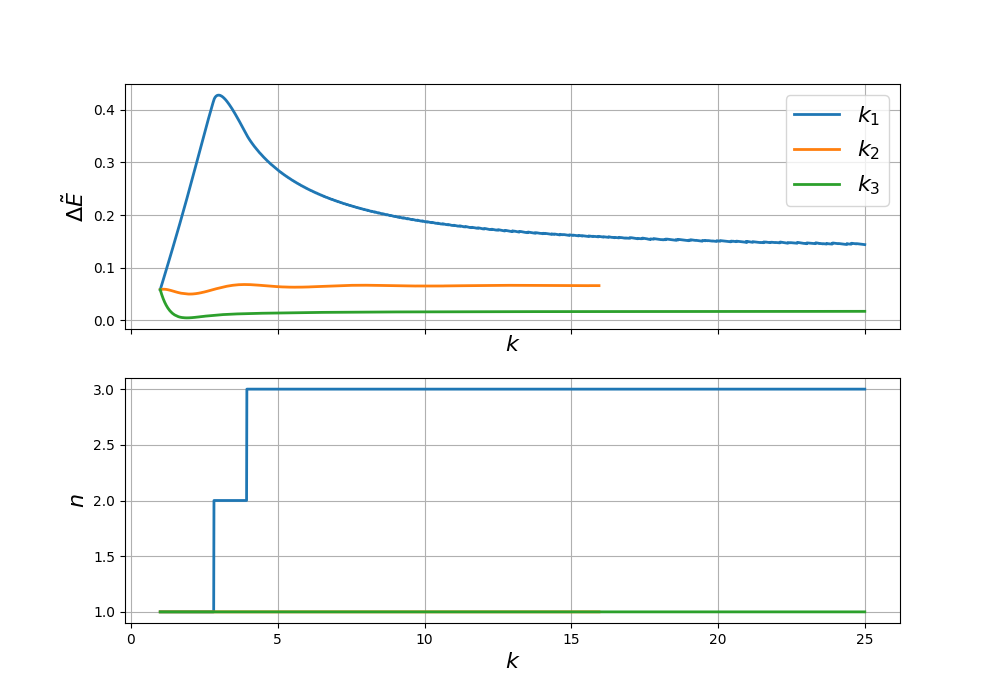
\includegraphics[width=0.7\textwidth]{stiff_deltas.png}
    \caption{Зависимость $\Delta \tilde{E}$ от различных значений жесткости пружин. Каждый график соответствует одной переменной массе. Нижний график демонстрирует зависимость количества соударений со стенкой от жесткости.}
    \label{fig:stiff_deltas}
\end{figure}

На первом графике на рисунке \ref{fig:stiff_deltas} видно, что $\Delta \tilde{E}$ сильнее всего зависит от значения жесткости первой пружины. При этом значение $\Delta \tilde{E}$ линейно достигает максимума, а затем логарифмически убывает. На нижнем графике продемонстрировано количество ударов о стенку в зависимости от жесткости пружины, важно заметить, что количество соударений зависят только от жесткости $k_1$. На основе рисунка \ref{fig:stiff_deltas}  можно сделать вывод, что максимальные значения $\Delta \tilde{E}$ находятся при значении $n=2$. При этом можно заметить, что значение жесткости $k_2$ практически не влияет на состояние системы, а увеличение значения жесткости $k_3$, наоборот приводят к уменьшению $\Delta \tilde{E}$, а следовательно и накопленной системой энергии.

Рассмотрим поведение системы для двух переменных параметров, для определения значений $\Delta \tilde{E}$.
Для этого построим срезы по различным плоскостям шестимерного пространства значений $k_1 k_2 k_3 m_1 m_2 m_3$. 
Белые области на графиках обозначают нефизические случаи. Для того чтобы избавиться от нефизических случаев было решено увеличить длну пружин и 
принять ее значение $l=10$.

\begin{figure}[b!]
    \begin{minipage}[h]{0.5\linewidth}
        \center{
            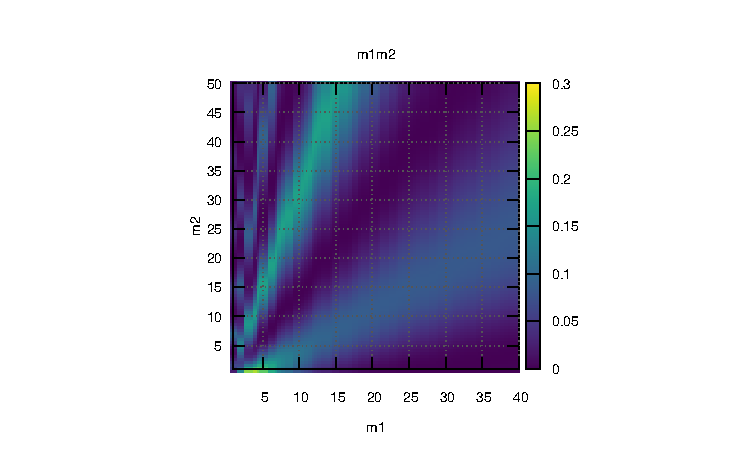
\includegraphics[width=1\textwidth]{m1m2.pdf} \\ a)
        }
    \end{minipage}
    \hfill
    \begin{minipage}[h]{0.5\linewidth}
        \center{
            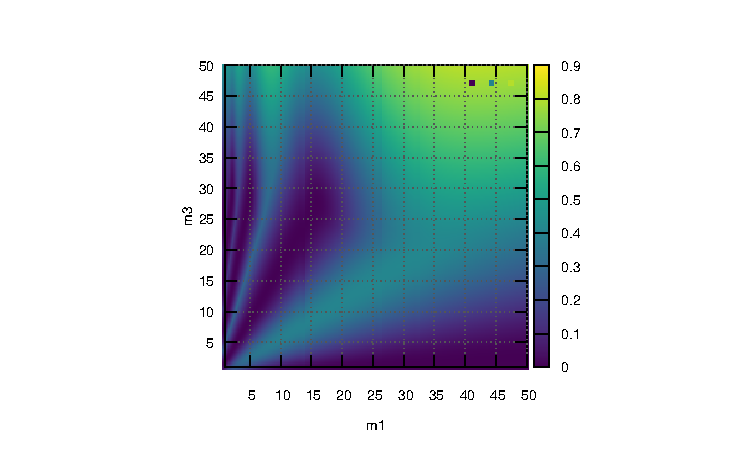
\includegraphics[width=1\textwidth]{m1m3.pdf} \\ б)
        }
    \end{minipage}
    \begin{center}
        \begin{minipage}[h]{0.5\linewidth}
            \center{
                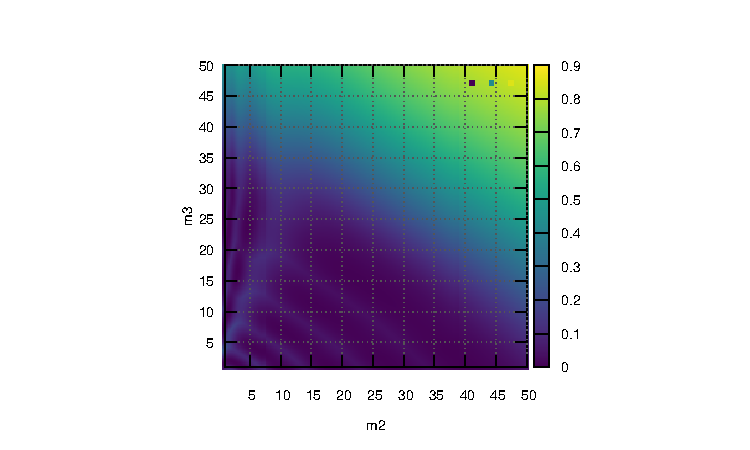
\includegraphics[width=1\textwidth]{m2m3.pdf} \\ в)
            }
        \end{minipage}
    \end{center}
    \caption{Срезы значений $\Delta \tilde{E}$ для двух переменных масс: $m_1$ $m_2$ (а), $m_1$ $m_3$ (б), $m_2$ $m_3$ (в). $l =10$ Фиксированные жесктости и массы =1}
    \label{fig:var2mass}
\end{figure}

\begin{figure}[b!]
    \begin{minipage}[h]{0.5\linewidth}
        \center{
            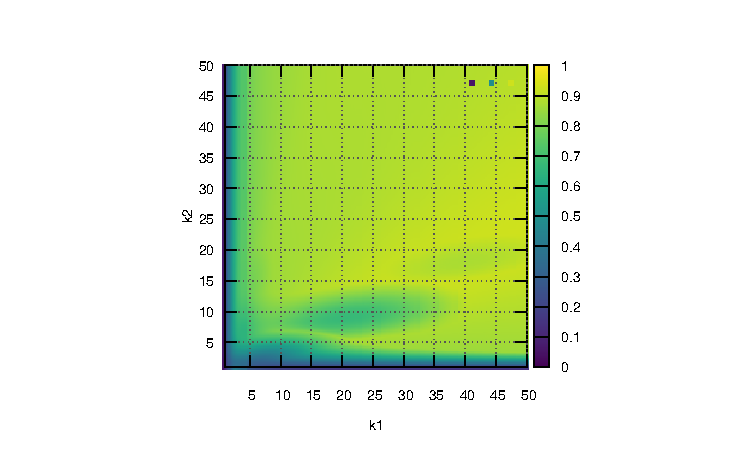
\includegraphics[width=1\textwidth]{k1k2.pdf} \\ a)
        }
    \end{minipage}
    \hfill
    \begin{minipage}[h]{0.5\linewidth}
        \center{
            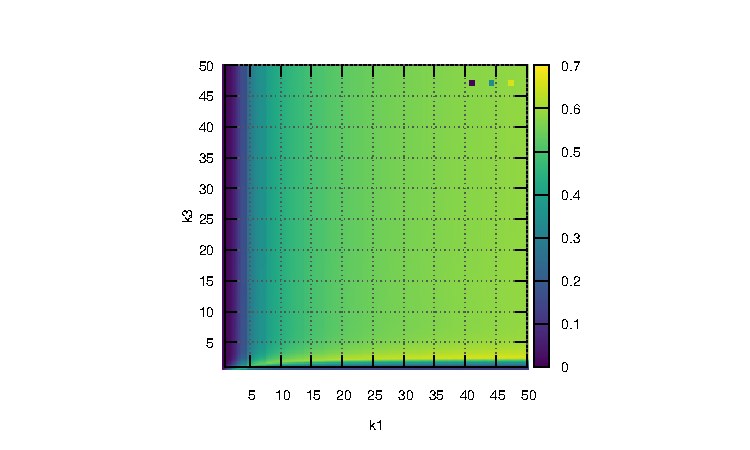
\includegraphics[width=1\textwidth]{k1k3.pdf} \\ б)
        }
    \end{minipage}
    \begin{center}
        \begin{minipage}[h]{0.5\linewidth}
            \center{
                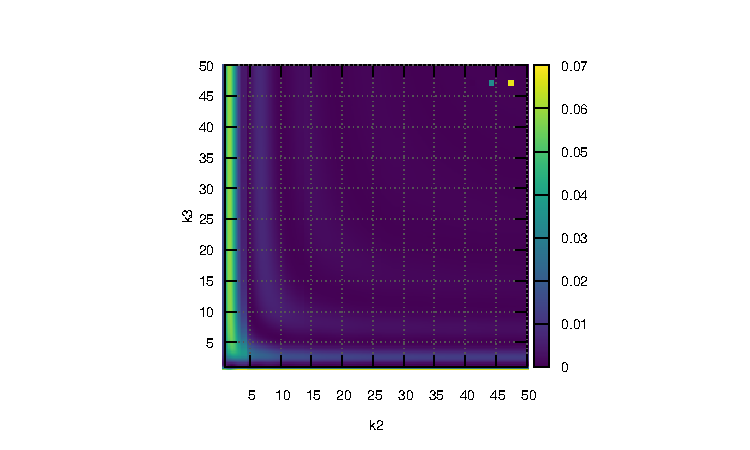
\includegraphics[width=1\textwidth]{k2k3.pdf} \\ в)
            }
        \end{minipage}
    \end{center}
    \caption{Срезы значений $\Delta \tilde{E}$ для двух переменных жесткостей: $k_1$ $k_2$ (а), $k_1$ $k_3$ (б), $k_2$ $k_3$ (в). $l =10$ Фиксированные жесткости и массы =1}
    \label{fig:var2stiff}
\end{figure}



\begin{figure}[b!]
    \begin{minipage}[h]{0.3\linewidth}
        \center{
            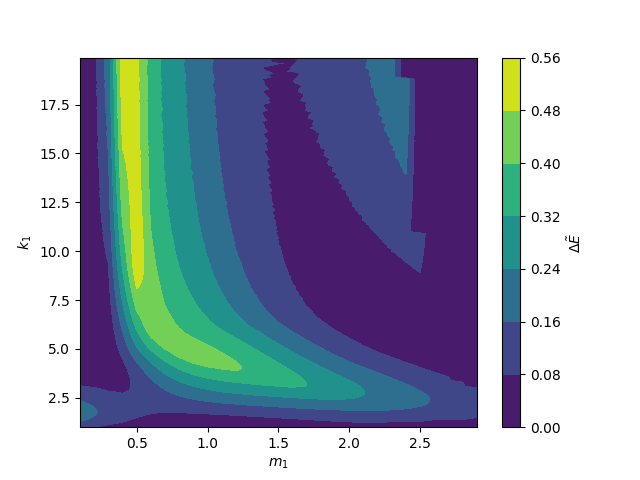
\includegraphics[width=1\textwidth]{m1k1.png} \\ a)
        }
    \end{minipage}
    \hfill
    \begin{minipage}[h]{0.3\linewidth}
        \center{
            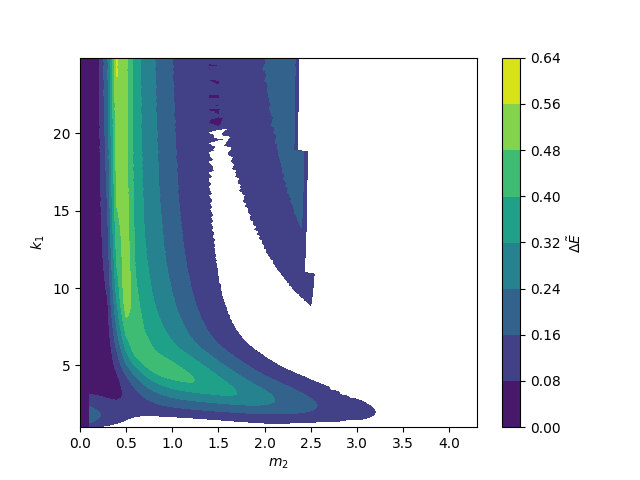
\includegraphics[width=1\textwidth]{m2k1.png} \\ б)
        }
    \end{minipage}
    \begin{minipage}[h]{0.3\linewidth}
        \center{
            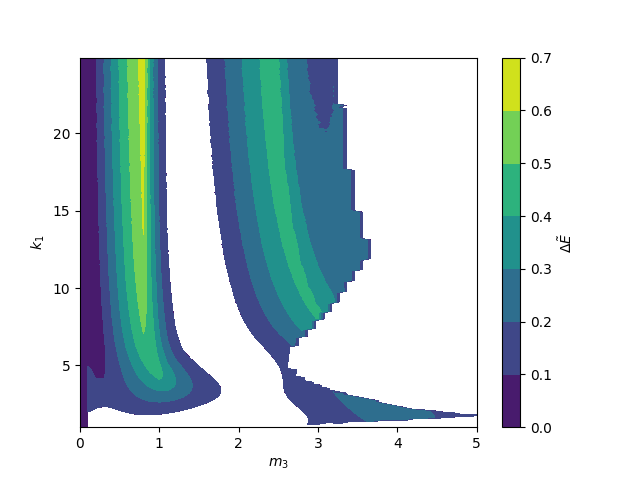
\includegraphics[width=1\textwidth]{m3k1.png} \\ в)
        }
    \end{minipage}
    \caption{Срезы значений $\Delta \tilde{E}$ для переменной жесткости $k_1$ и переменной массы: $m_1$ (а), $m_2$ (б), $m_3$ (в)}
    \label{fig:var2k1}
\end{figure}


\begin{figure}[b!]
    \begin{minipage}[h]{0.3\linewidth}
        \center{
            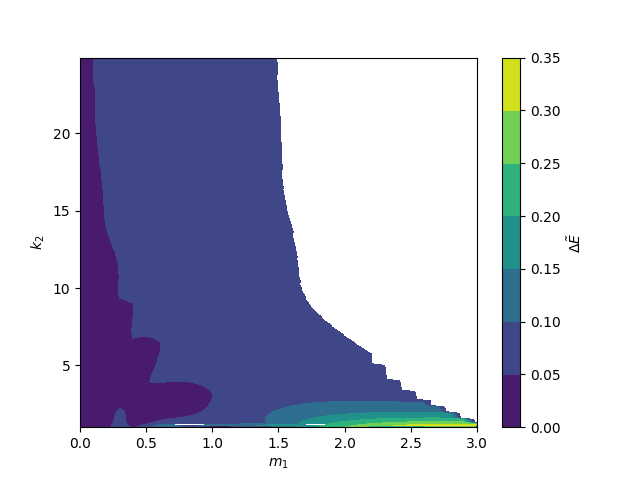
\includegraphics[width=1\textwidth]{m1k2.png} \\ a)
        }
    \end{minipage}
    \hfill
    \begin{minipage}[h]{0.3\linewidth}
        \center{
            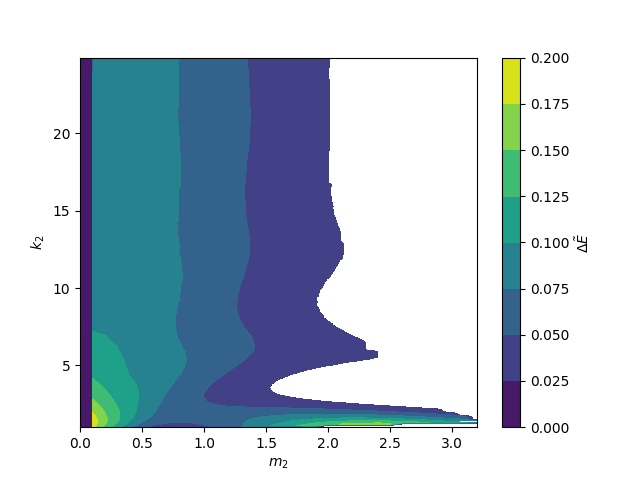
\includegraphics[width=1\textwidth]{m2k2.png} \\ б)
        }
    \end{minipage}
    \begin{minipage}[h]{0.3\linewidth}
        \center{
            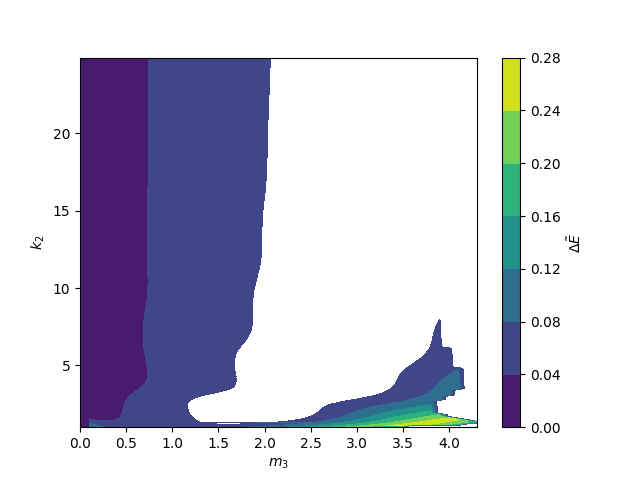
\includegraphics[width=1\textwidth]{m3k2.png} \\ в)
        }
    \end{minipage}
    \caption{Срезы значений $\Delta \tilde{E}$ для переменной жесткости $k_2$ и переменной массы: $m_1$ (а), $m_2$ (б), $m_3$ (в). Цветом обозначена величина накопленной энергии}
    \label{fig:var2k2}
\end{figure}


\begin{figure}[b!]
    \begin{minipage}[h]{0.3\linewidth}
        \center{
            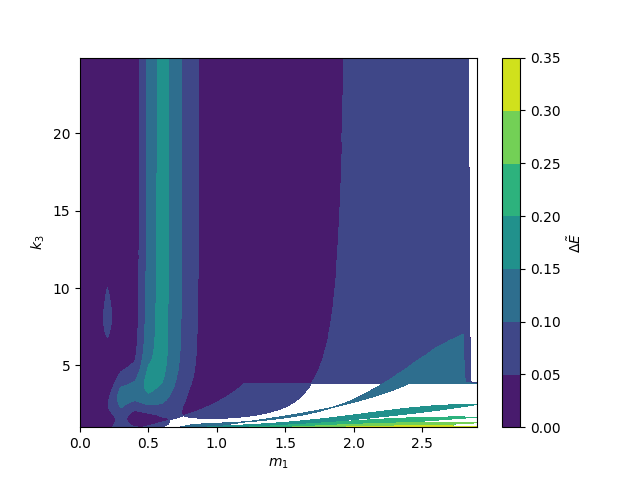
\includegraphics[width=1\textwidth]{m1k3.png} \\ a)
        }
    \end{minipage}
    \hfill
    \begin{minipage}[h]{0.3\linewidth}
        \center{
            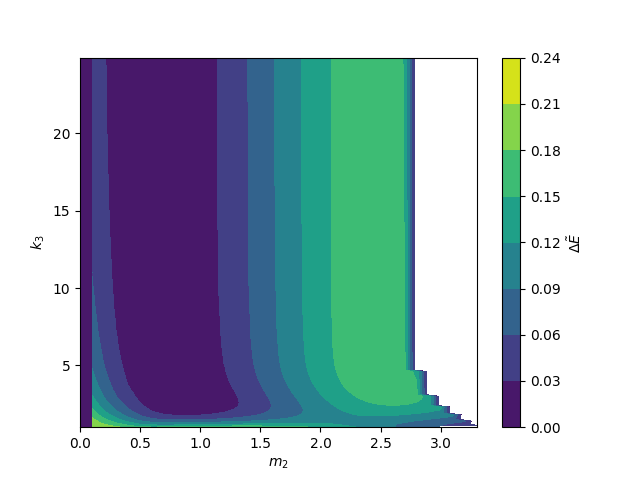
\includegraphics[width=1\textwidth]{m2k3.png} \\ б)
        }
    \end{minipage}
    \begin{minipage}[h]{0.3\linewidth}
        \center{
            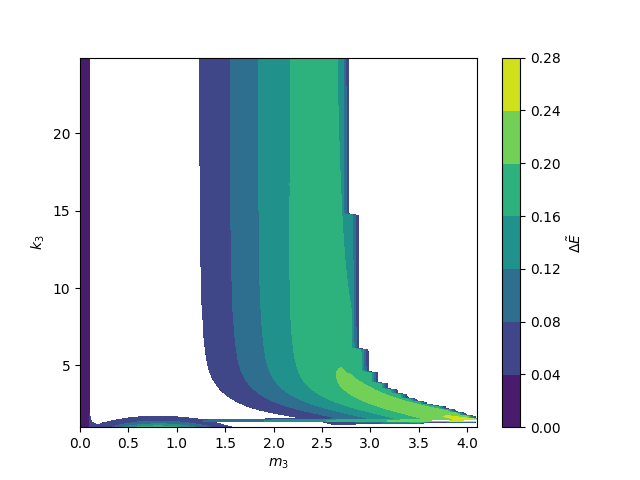
\includegraphics[width=1\textwidth]{m3k3.png} \\ в)
        }
    \end{minipage}
    \caption{Срезы значений $\Delta \tilde{E}$ для переменной жесткости $k_3$ и переменной массы: $m_1$ (а), $m_2$ (б), $m_3$ (в). }
    \label{fig:var2k3}
\end{figure}


Полученные срезы позволяют понять какие переменные вносят больший вклад в диссипацию энергии в системе. Но данная выборка не может считаться полностью репрезентативной, так как в большинстве случаев области значений подобраны таким образом чтобы ограничить область нефизических случаев. Но даже такие данные позволяют сделать некоторые выводы насчет поведения системы. В частности на рисунке \ref{fig:var2mass} можно увидеть периодичность максимумов, при этом для графиков (a) и (б) она зависит от $tg \alpha$ равное соотношению масс. Для графика (в), область оптимальных значений находится в области $m_3 \rightarrow min$, но в то же время максимумы чередуются в зависимости от значения $m_2$. Что позволяет сделать вывод, о том что $\Delta \tilde{E}$ зависит в большей степени не от значений масс системы, а от их отношения.

При этом если рассматривать графики, изображенные на рисунке \ref{fig:var2stiff}, то можно легко заметить по графикам (а) и (б), что
$\Delta \tilde{E}$ практически не зависит от значений $k_2$ и $k_3$, но при этом линейно зависят от значений $k_1$. Основной вклад в диссипацию энергии вносит первая пружина, а на по графику (в) видно что при минимизации жесткости $k_2$ происходит увеличение $\Delta \tilde{E}$, что соответствует данным, полученным на графике (а).

На рисунке \ref{fig:var2k1} можно увидеть, что $\Delta \tilde{E} \rightarrow max$ при определенных значениях массы и линейно зависят от $k_1$ в окрестностях оптимальной массы. Так же можно предположить некоторую периодичность процесса, но по причине того, что для данных переменных, система достаточно быстро переходит в нефизическое состояние, то делать сложно делать какие либо однозначные выводы.

Рисунки  \ref{fig:var2k2} и \ref{fig:var2k3} демонстрируют зависимость $\Delta \tilde{E}$ для переменных масс и жесткостей $k_2$ и $k_3$ соответственно. Но легко можно заметить, что максимальные значения $\Delta \tilde{E}$ находятся на границе с нефизическими состояниями системы. Скорей всего данные отношения не представляют какой либо практический интерес.

Контуры срезов, полученные на рисунках \ref{fig:var2mass} - \ref{fig:var2k3} соответствуют данным, полученным на рисунках \ref{fig:deltas} и \ref{fig:stiff_deltas}. На графиках присутствует периодичность для масс, которую можно заметить и на полученных срезах, а так же видна линейная зависимость $\Delta \tilde{E}$ от $k_1$.

Рассмотрим трехмерные пространства изменяемых параметров масс и жесткостей пружин. Для этого провердем численный эксперимент для каждого значения массы
с выбранным шагом($h=0.5$), и получим облака точек, изображенные на рисунке \ref{fig:3d}, значения накопленной энергии в которых, обозначено цветом.


\begin{figure}[b!]
    \centering
    \begin{minipage}[h]{0.49\linewidth}
        \center{
           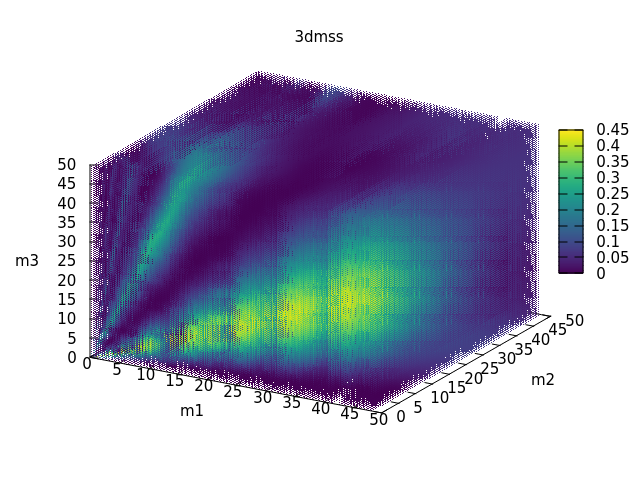
\includegraphics[width=1\textwidth]{3dmssnew.png} \\ a)
        }
    \end{minipage}
    \hfill
    \begin{minipage}[h]{0.49\linewidth}
        \center{
           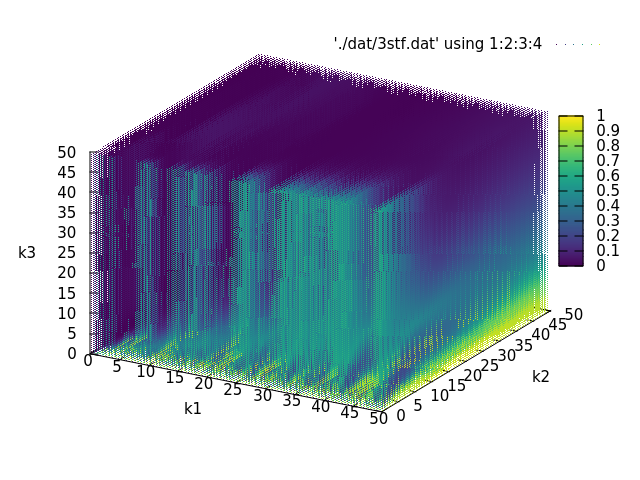
\includegraphics[width=1\textwidth]{3dstfs.png} \\ б)
        }
    \end{minipage}
    \caption{Зависимость $\Delta \tilde{E}$ от различных значений масс (a) и различных значений жесткостей (б). Значение $\Delta \tilde{E}$ указано цветом.}
    \label{fig:3d}
\end{figure}

Так как сами по себе графики представленные на рисунке \ref{fig:3d} не очень репрезентативны, то построим графики содержащие только точки в которых значение $\Delta \tilde{E} < 0.01$. 
точек, отображающие зоны минимальных и максимальных накопленных энергий. 

\begin{figure}[b!]
    \centering
    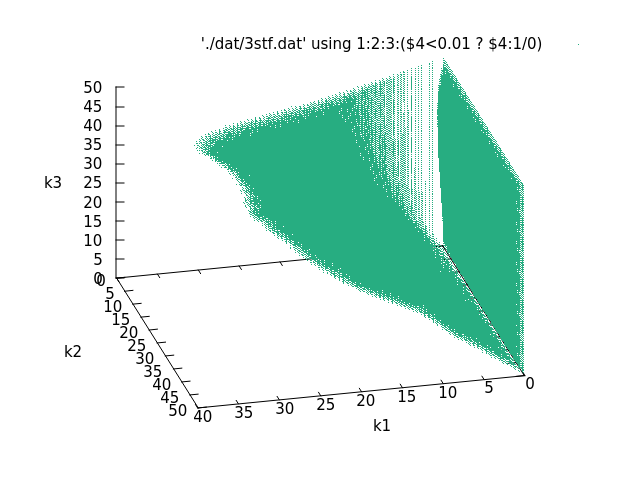
\includegraphics{stfsmin.png}
    \caption{Области $\Delta \tilde{E} < 0.01$  для переменных жесктостей}
    \label{minmss3d}
\end{figure}


\begin{figure}[b!]
    \centering
    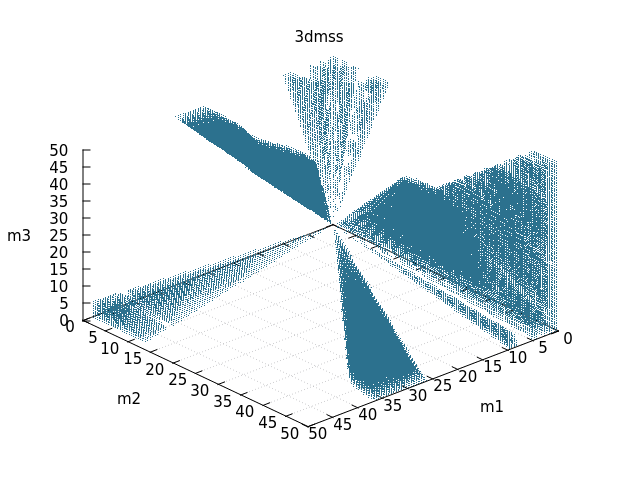
\includegraphics{3dmssmin.png}
    \caption{Области $\Delta \tilde{E} < 0.01$  для переменных масс}
    \label{minmss3d}
\end{figure}

\begin{figure}[b!]
    \centering
    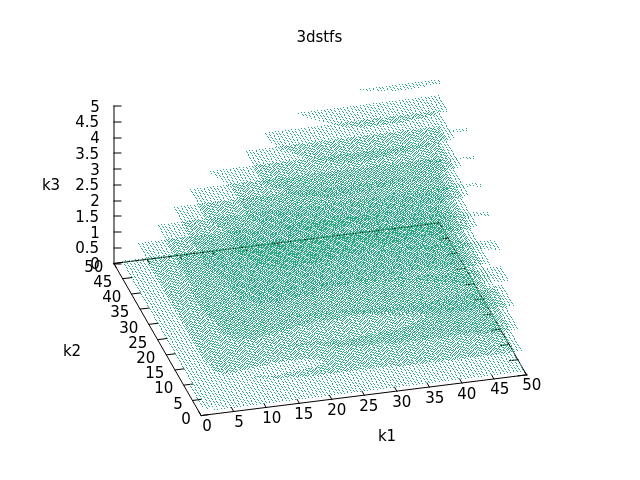
\includegraphics{3dstfsmax.png}
    \caption{Области максимальных значений $\Delta \tilde{E}$  для переменных жесткостей}
    \label{minmss3d}
\end{figure}

\newpage
\begin{figure}[b!]
    \centering
    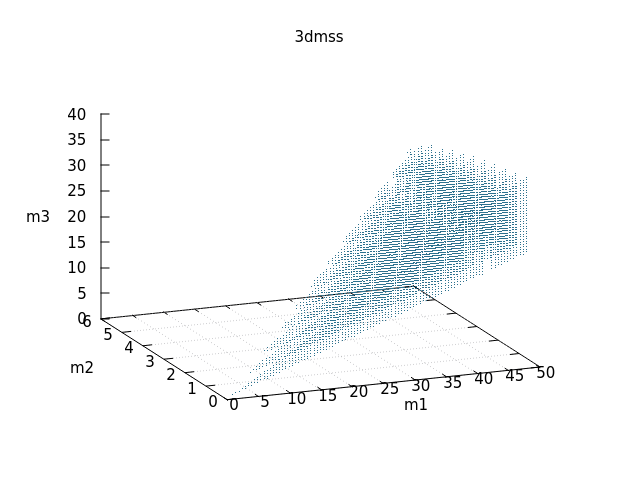
\includegraphics{3dmssmax.png}
    \caption{Области максимальных значений $\Delta \tilde{E}$  для переменных масс}
    \label{minmss3d}
\end{figure}

Посторим траектории системы трех тел в полученных областях максимальных и минимальных энергий. Полученные траектории могут продемонстрировать механизмы перехода
энергии с макроуровня на микроуровень.

\begin{figure}[t!]
    \centering
    \centering
    \begin{minipage}[h]{0.49\linewidth}
        \center{
           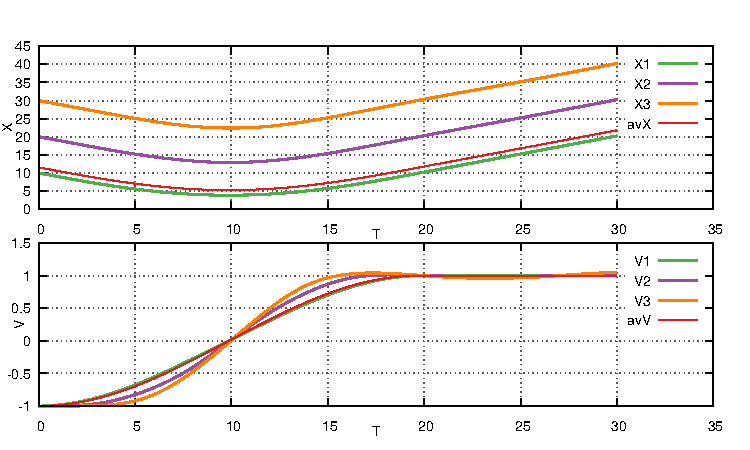
\includegraphics[width=1\textwidth]{tr/trbigm1.pdf} \\ a)
        }
    \end{minipage}
    \hfill
    \begin{minipage}[h]{0.49\linewidth}
        \center{
           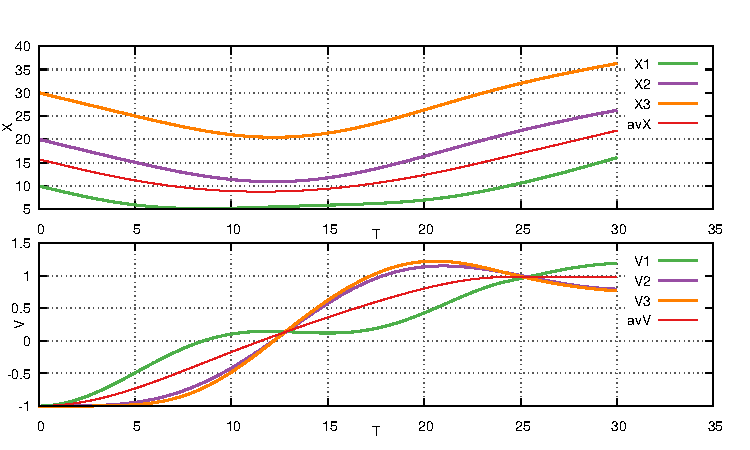
\includegraphics[width=1\textwidth]{tr/trbigm1m2.pdf} \\ б)
        }
    \end{minipage}
    \begin{minipage}[h]{0.49\linewidth}
        \center{
           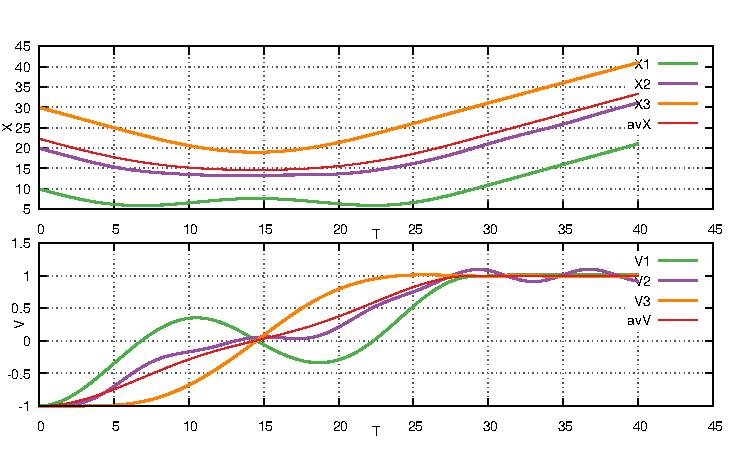
\includegraphics[width=1\textwidth]{tr/trbigm1m3.pdf} \\ в)
        }
    \end{minipage}
    \begin{minipage}[h]{0.49\linewidth}
        \center{
           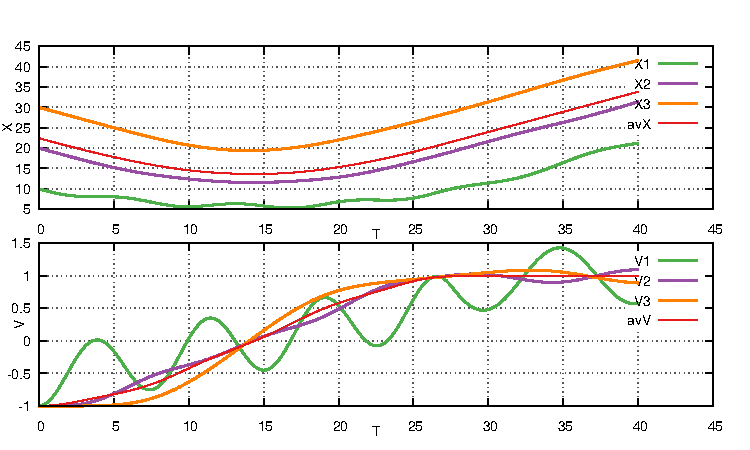
\includegraphics[width=1\textwidth]{tr/trbigm2m3.pdf} \\ г)
        }
    \end{minipage}
    \begin{minipage}[h]{0.49\linewidth}
        \center{
           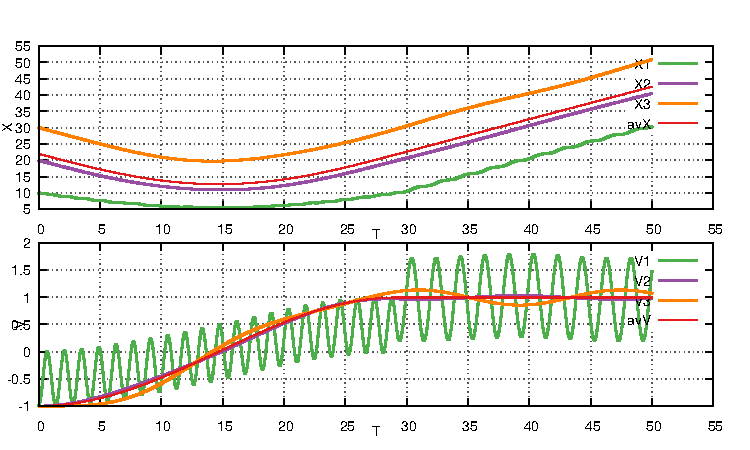
\includegraphics[width=1\textwidth]{tr/trmink.pdf} \\ д)
        }
    \end{minipage}
    \caption{Траектории тела, при которых  $\Delta \tilde{E}$ минимальна. a) $m_1$ значительно больше остальных масс б) $m_1>>m_3$, $m_2>>m_3$\\
    в) $m_1>>m_2$, $m_3>>m_1$, г) $m_2>>m_1$, $m_2>>m_3$, д) $k_1 \rightarrow 0$ }
    \label{fig:mintr}
\end{figure}


\begin{figure}[t!]
    \centering
    \centering
    \begin{minipage}[h]{0.49\linewidth}
        \center{
           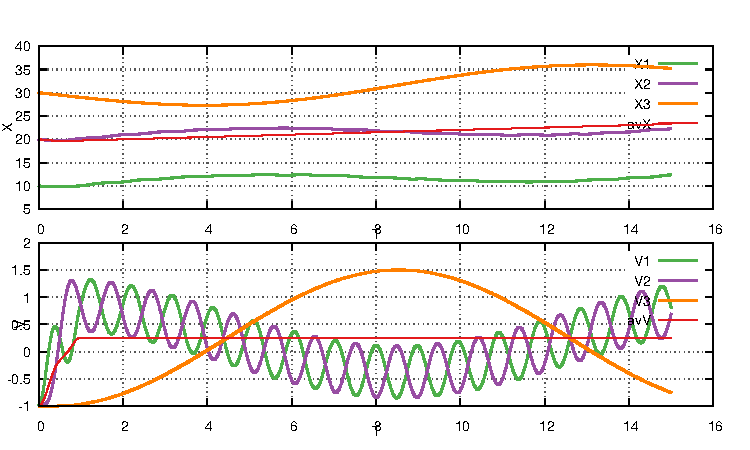
\includegraphics[width=1\textwidth]{tr/trmaxstfs.pdf} \\ a)
        }
    \end{minipage}
    \begin{minipage}[h]{0.49\linewidth}
        \center{
           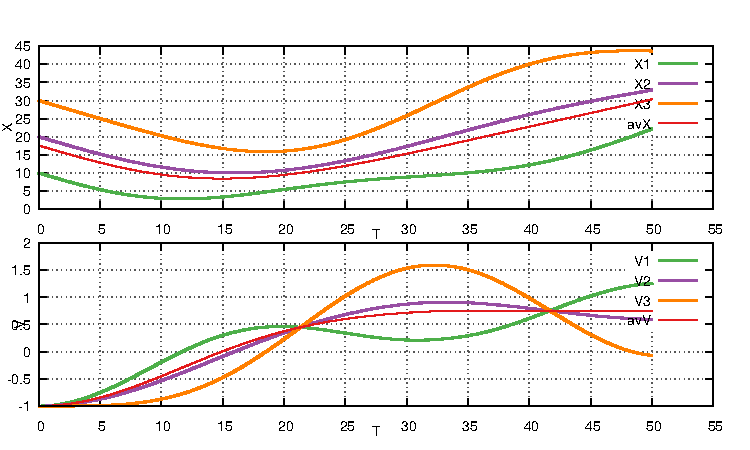
\includegraphics[width=1\textwidth]{tr/trlilm2.pdf} \\ б)
        }
    \end{minipage}
    \caption{Траектории тела, при которой  $\Delta \tilde{E}$ максимальна а) для переменных жесткостей б) переменных масс}
    \label{fig:maxtr}
\end{figure}


На основе рисунков \ref{fig:mintr} и \ref{fig:maxtr} можно сделать вывод, что в предельных случаях система трех тел сводится к системе двух тел.
Значение диссипации будет зависеть от того каким образом система из трех тел преобразуется в систему двух тел при взаимодействии. 

Для максимума накопленной энергии система преобразуется в систему двух тел, в которой одно тело представляет из себя два тела, которые совершают гармонические колебания относительно общего
центра масс. Данный центр масс в свою очередь будет колебаться относительно оставшейся массы. Такая конфигурация позволяет преобразовать наибольшее количество
кинетической энергии тела на макроуровне во внутреннюю энергию тела.

В случае минимума наколенной энергии система стремится к единому абсолютно упругому телу, такие конфигурации сводятся к случаям, когда одна масса является
максимальной и вклад от других масс не является значительным. Так же есть случаи когда две массы совершают гармонические колебания, но третья масса является 
столь незначительной, либо засчет жесткости пружин не может внести достаточного вклада в данную систему. 


\backmatter %% Здесь заканчивается нумерованная часть документа и начинаются ссылки и
            

%:Заключение
\chapter{ЗАКЛЮЧЕНИЕ}

В ходе работы были выполнены следующие задачи:
\begin{itemize}
	\item По теме "Силовые сети в гранулированных средах" был проведен обзор литературы и было обнаружено отсутствие подходящих исследований, описывающих проблематику проекта
	\item Определена актуальность проекта и определена цель исследования в соответствии с актуальными вопросами по теме проекта
	\item Составлена математическая модель неабсолютно упругого соударения системы трех тел со стенкой.
	\item Построен и реализован конечный автомат, описывающий состояния системы.
	\item Проведен анализ методов решения и выбор оптимального. 
	\begin{itemize}
		\item Реализовано аналитическое решение системы ОДУ
		\item Реализован метод Рунге-Кутта для решения ОДУ
		\item Произведен анализ эффективности методов и скорости расчетов.
	\end{itemize}
	\item Проведен анализ зависимости коэффициента эффективности диссипации от значений переменных системы.
	\begin{itemize}
		\item Были построены двумерные и трехмерные облака точек, показывающие зависимости коэффициента диссипации от параметров системы
		\item Определены принципы поведения системы трех тел в областях максимумов и минимумов энергий.  
	\end{itemize}
\end{itemize}

Данные, полученные в ходе работы над курсовым проектом, являются стартовой точкой для понимания процессов, происходящих в неабсолютно упругих телах при соударении. Данная математическая модель и понимание какие из параметров сильней всего влияют на состояние системы, позволят в дальнейшем найти такие значения параметров системы для которых накопленная внутренняя энергия будет максимальна, что позволит определить оптимальные параметры для полидисперсных демпфирующих систем. 
%% заключение

\bibliographystyle{gost2008}
\bibliography{bib/grnbib}


\appendix   % Тут идут приложения
\chapter{ПРИЛОЖЕНИЯ}

\end{document}

%%% Local Variables:
%%% mode: latex
%%% TeX-master: t
%%% End:
